\documentclass[a4paper]{book}
\usepackage{makeidx}
\usepackage{natbib}
\usepackage{graphicx}
\usepackage{multicol}
\usepackage{float}
\usepackage{listings}
\usepackage{color}
\usepackage{ifthen}
\usepackage[table]{xcolor}
\usepackage{textcomp}
\usepackage{alltt}
\usepackage{ifpdf}
\ifpdf
\usepackage[pdftex,
            pagebackref=true,
            colorlinks=true,
            linkcolor=blue,
            unicode
           ]{hyperref}
\else
\usepackage[ps2pdf,
            pagebackref=true,
            colorlinks=true,
            linkcolor=blue,
            unicode
           ]{hyperref}
\usepackage{pspicture}
\fi
\usepackage[utf8]{inputenc}
\usepackage{mathptmx}
\usepackage[scaled=.90]{helvet}
\usepackage{courier}
\usepackage{sectsty}
\usepackage[titles]{tocloft}
\usepackage{doxygen}
\lstset{language=C++,inputencoding=utf8,basicstyle=\footnotesize,breaklines=true,breakatwhitespace=true,tabsize=8,numbers=left }
\makeindex
\setcounter{tocdepth}{3}
\renewcommand{\footrulewidth}{0.4pt}
\renewcommand{\familydefault}{\sfdefault}
\hfuzz=15pt
\setlength{\emergencystretch}{15pt}
\hbadness=750
\tolerance=750
\begin{document}
\hypersetup{pageanchor=false,citecolor=blue}
\begin{titlepage}
\vspace*{7cm}
\begin{center}
{\Large \-Smoothed \-Particle \-Hydrodynamics }\\
\vspace*{1cm}
{\large \-Generated by Doxygen 1.7.6.1}\\
\vspace*{0.5cm}
{\small Fri Jan 18 2013 11:11:19}\\
\end{center}
\end{titlepage}
\clearemptydoublepage
\pagenumbering{roman}
\tableofcontents
\clearemptydoublepage
\pagenumbering{arabic}
\hypersetup{pageanchor=true,citecolor=blue}
\chapter{\-Main \-Page}
\label{index}\hypertarget{index}{}\-This is where the overview of the program goes. \-Need to write that. 
\chapter{\-Class \-Index}
\section{\-Class \-Hierarchy}
\-This inheritance list is sorted roughly, but not completely, alphabetically\-:\begin{DoxyCompactList}
\item \contentsline{section}{\-Fluid}{\pageref{classFluid}}{}
\item \contentsline{section}{\-Integrator}{\pageref{classIntegrator}}{}
\begin{DoxyCompactList}
\item \contentsline{section}{\-Euler}{\pageref{classEuler}}{}
\end{DoxyCompactList}
\item \contentsline{section}{\-Kernel}{\pageref{classKernel}}{}
\begin{DoxyCompactList}
\item \contentsline{section}{\-Gaussian\-Kernel}{\pageref{classGaussianKernel}}{}
\item \contentsline{section}{\-Spline\-Kernel}{\pageref{classSplineKernel}}{}
\end{DoxyCompactList}
\item \contentsline{section}{\-Kvector}{\pageref{structKvector}}{}
\item \contentsline{section}{\-Output}{\pageref{classOutput}}{}
\item \contentsline{section}{\-Particle}{\pageref{classParticle}}{}
\item \contentsline{section}{\-Physics}{\pageref{classPhysics}}{}
\begin{DoxyCompactList}
\item \contentsline{section}{\-Incomp\-Invisc}{\pageref{classIncompInvisc}}{}
\end{DoxyCompactList}
\item \contentsline{section}{\-Properties}{\pageref{structProperties}}{}
\end{DoxyCompactList}

\chapter{\-Class \-Index}
\section{\-Class \-List}
\-Here are the classes, structs, unions and interfaces with brief descriptions\-:\begin{DoxyCompactList}
\item\contentsline{section}{\hyperlink{classEuler}{\-Euler} \\*\hyperlink{classEuler}{\-Euler} integrator }{\pageref{classEuler}}{}
\item\contentsline{section}{\hyperlink{classFluid}{\-Fluid} \\*\-Holds particles and boundary praticles }{\pageref{classFluid}}{}
\item\contentsline{section}{\hyperlink{classGaussianKernel}{\-Gaussian\-Kernel} \\*\-Gaussian approximation of point particle }{\pageref{classGaussianKernel}}{}
\item\contentsline{section}{\hyperlink{classIncompInvisc}{\-Incomp\-Invisc} \\*\-Class for an incompressibe, inviscid fluid }{\pageref{classIncompInvisc}}{}
\item\contentsline{section}{\hyperlink{classIncompVisc}{\-Incomp\-Visc} \\*\-Class for an incompressible fluid with the inclusion of viscous forces }{\pageref{classIncompVisc}}{}
\item\contentsline{section}{\hyperlink{classIntegrator}{\-Integrator} \\*\-Superclass for integrators }{\pageref{classIntegrator}}{}
\item\contentsline{section}{\hyperlink{classKernel}{\-Kernel} \\*\-Smooth kernels approximating point particles }{\pageref{classKernel}}{}
\item\contentsline{section}{\hyperlink{structKvector}{\-Kvector} \\*\-Struct for 2\-D vector useful for kernel operations }{\pageref{structKvector}}{}
\item\contentsline{section}{\hyperlink{classOutput}{\-Output} \\*\-Class to build output file for fluid state }{\pageref{classOutput}}{}
\item\contentsline{section}{\hyperlink{classParticle}{\-Particle} \\*\hyperlink{structProperties}{\-Properties} and functions for individual particles }{\pageref{classParticle}}{}
\item\contentsline{section}{\hyperlink{classPhysics}{\-Physics} \\*\-Superclass for implementing different fluid physics }{\pageref{classPhysics}}{}
\item\contentsline{section}{\hyperlink{classPredictorCorrector}{\-Predictor\-Corrector} \\*\-Predictor-\/corrector integrator }{\pageref{classPredictorCorrector}}{}
\item\contentsline{section}{\hyperlink{structProperties}{\-Properties} \\*\-Struct holding physical particle properties }{\pageref{structProperties}}{}
\item\contentsline{section}{\hyperlink{classSplineKernel}{\-Spline\-Kernel} \\*\-Cubic spline approximation of point particle }{\pageref{classSplineKernel}}{}
\end{DoxyCompactList}

\chapter{\-File \-Index}
\section{\-File \-List}
\-Here is a list of all documented files with brief descriptions\-:\begin{DoxyCompactList}
\item\contentsline{section}{\hyperlink{euler_8h}{euler.\-h} \\*\-Implementation of explicit \hyperlink{classEuler}{\-Euler} integrator }{\pageref{euler_8h}}{}
\item\contentsline{section}{\hyperlink{eulermod_8h}{eulermod.\-h} \\*\-Implementation of \hyperlink{classEuler}{\-Euler} integrator, modified so that the position is updated using the updated velocity }{\pageref{eulermod_8h}}{}
\item\contentsline{section}{\hyperlink{fluid_8h}{fluid.\-h} \\*\-Definition of fluid class for packaging together particles, boundary particles, and their properties }{\pageref{fluid_8h}}{}
\item\contentsline{section}{\hyperlink{fluid__test_8cc}{fluid\-\_\-test.\-cc} \\*\-Tests for \hyperlink{classFluid}{\-Fluid} }{\pageref{fluid__test_8cc}}{}
\item\contentsline{section}{\hyperlink{gaussiankernel_8h}{gaussiankernel.\-h} \\*\-Implementation of a \-Gaussian kernel }{\pageref{gaussiankernel_8h}}{}
\item\contentsline{section}{\hyperlink{incompinvisc_8h}{incompinvisc.\-h} \\*\-Implementation of \hyperlink{classPhysics}{\-Physics} for a fluid which is incompressible and inviscid }{\pageref{incompinvisc_8h}}{}
\item\contentsline{section}{\hyperlink{incompvisc_8h}{incompvisc.\-h} \\*\-Implementation of \hyperlink{classPhysics}{\-Physics} for a fluid which is incompressible and viscous }{\pageref{incompvisc_8h}}{}
\item\contentsline{section}{\hyperlink{initialize_8h}{initialize.\-h} \\*\-Code for initialization of fluid and boundary from input files }{\pageref{initialize_8h}}{}
\item\contentsline{section}{\hyperlink{integrator_8h}{integrator.\-h} \\*\-Superclass for integrators }{\pageref{integrator_8h}}{}
\item\contentsline{section}{\hyperlink{kernel_8h}{kernel.\-h} \\*\-Superclass for kernels }{\pageref{kernel_8h}}{}
\item\contentsline{section}{\hyperlink{kernel__test_8cc}{kernel\-\_\-test.\-cc} \\*\-Tests \hyperlink{classSplineKernel}{\-Spline\-Kernel} and \hyperlink{classGaussianKernel}{\-Gaussian\-Kernel} }{\pageref{kernel__test_8cc}}{}
\item\contentsline{section}{\hyperlink{kvector_8h}{kvector.\-h} \\*\-Struct for 2\-D vector object useful for kernel operations }{\pageref{kvector_8h}}{}
\item\contentsline{section}{\hyperlink{kvector__test_8cc}{kvector\-\_\-test.\-cc} \\*\-Tests for \hyperlink{structKvector}{\-Kvector} }{\pageref{kvector__test_8cc}}{}
\item\contentsline{section}{\hyperlink{output_8h}{output.\-h} \\*\-Class which outputs current fluid state }{\pageref{output_8h}}{}
\item\contentsline{section}{\hyperlink{particle_8h}{particle.\-h} \\*\-Definition of the particle class }{\pageref{particle_8h}}{}
\item\contentsline{section}{\hyperlink{particle__test_8cc}{particle\-\_\-test.\-cc} \\*\-Tests \hyperlink{classParticle}{\-Particle} }{\pageref{particle__test_8cc}}{}
\item\contentsline{section}{\hyperlink{physics_8h}{physics.\-h} \\*\-Superclass for implementing different fluid physics }{\pageref{physics_8h}}{}
\item\contentsline{section}{\hyperlink{predictorcorrector_8h}{predictorcorrector.\-h} \\*\hyperlink{classIntegrator}{\-Integrator} implimenting the modified predictor-\/corrector method outlined in \-Price (2004) }{\pageref{predictorcorrector_8h}}{}
\item\contentsline{section}{\hyperlink{properties_8h}{properties.\-h} \\*\-Struct to hold a particle's physical properties }{\pageref{properties_8h}}{}
\item\contentsline{section}{\hyperlink{properties__test_8cc}{properties\-\_\-test.\-cc} \\*\-Tests for \hyperlink{structProperties}{\-Properties} }{\pageref{properties__test_8cc}}{}
\item\contentsline{section}{\hyperlink{sph_8cc}{sph.\-cc} \\*\-Driver program for smoothed particle hydrodynamics solver }{\pageref{sph_8cc}}{}
\item\contentsline{section}{\hyperlink{splinekernel_8h}{splinekernel.\-h} \\*\-Implentation of a cubic spline kernel }{\pageref{splinekernel_8h}}{}
\item\contentsline{section}{\hyperlink{tests_8cc}{tests.\-cc} \\*\-Driver program for testing of sph }{\pageref{tests_8cc}}{}
\end{DoxyCompactList}

\chapter{\-Class \-Documentation}
\hypertarget{classEuler}{\section{\-Euler \-Class \-Reference}
\label{classEuler}\index{\-Euler@{\-Euler}}
}


euler integrator  




{\ttfamily \#include $<$euler.\-h$>$}



\-Inheritance diagram for \-Euler\-:
\nopagebreak
\begin{figure}[H]
\begin{center}
\leavevmode
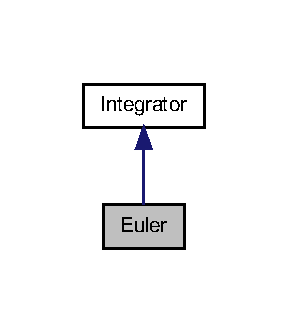
\includegraphics[width=138pt]{classEuler__inherit__graph}
\end{center}
\end{figure}


\-Collaboration diagram for \-Euler\-:
\nopagebreak
\begin{figure}[H]
\begin{center}
\leavevmode
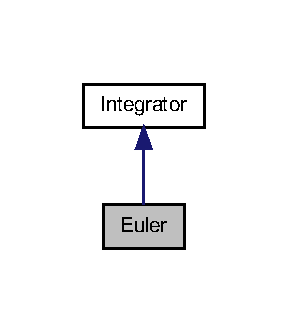
\includegraphics[width=138pt]{classEuler__coll__graph}
\end{center}
\end{figure}
\subsection*{\-Public \-Member \-Functions}
\begin{DoxyCompactItemize}
\item 
\hypertarget{classEuler_abae73a2536cea422aab8e6d637b766d7}{\hyperlink{classEuler_abae73a2536cea422aab8e6d637b766d7}{\-Euler} (double dt, \hyperlink{classFluid}{\-Fluid} \&fluid, \hyperlink{classPhysics}{\-Physics} \&physics)}\label{classEuler_abae73a2536cea422aab8e6d637b766d7}

\begin{DoxyCompactList}\small\item\em ctor \end{DoxyCompactList}\item 
\hypertarget{classEuler_a343d589f62a1073886e76c82e0689aed}{int \hyperlink{classEuler_a343d589f62a1073886e76c82e0689aed}{step} ()}\label{classEuler_a343d589f62a1073886e76c82e0689aed}

\begin{DoxyCompactList}\small\item\em advances one timestep \end{DoxyCompactList}\end{DoxyCompactItemize}


\subsection{\-Detailed \-Description}
euler integrator 

\-The documentation for this class was generated from the following file\-:\begin{DoxyCompactItemize}
\item 
\hyperlink{euler_8h}{euler.\-h}\end{DoxyCompactItemize}

\hypertarget{classEulermod}{\section{\-Eulermod \-Class \-Reference}
\label{classEulermod}\index{\-Eulermod@{\-Eulermod}}
}


modified \hyperlink{classEuler}{\-Euler} integrator  




{\ttfamily \#include $<$eulermod.\-h$>$}



\-Inheritance diagram for \-Eulermod\-:\nopagebreak
\begin{figure}[H]
\begin{center}
\leavevmode
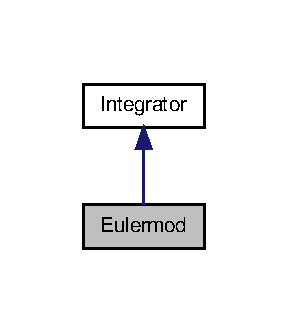
\includegraphics[width=138pt]{classEulermod__inherit__graph}
\end{center}
\end{figure}


\-Collaboration diagram for \-Eulermod\-:\nopagebreak
\begin{figure}[H]
\begin{center}
\leavevmode
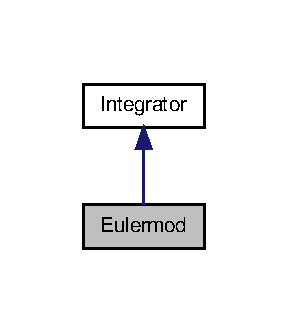
\includegraphics[width=138pt]{classEulermod__coll__graph}
\end{center}
\end{figure}
\subsection*{\-Public \-Member \-Functions}
\begin{DoxyCompactItemize}
\item 
\hypertarget{classEulermod_a60dfcac405d5024f76baa9f4cf037a18}{\hyperlink{classEulermod_a60dfcac405d5024f76baa9f4cf037a18}{\-Eulermod} (double dt, \hyperlink{classFluid}{\-Fluid} \&fluid, \hyperlink{classPhysics}{\-Physics} \&physics)}\label{classEulermod_a60dfcac405d5024f76baa9f4cf037a18}

\begin{DoxyCompactList}\small\item\em ctor \end{DoxyCompactList}\item 
\hypertarget{classEulermod_aa47d39f3d649484b159ecdd4b6d88ff2}{int \hyperlink{classEulermod_aa47d39f3d649484b159ecdd4b6d88ff2}{step} ()}\label{classEulermod_aa47d39f3d649484b159ecdd4b6d88ff2}

\begin{DoxyCompactList}\small\item\em advances one timestep \end{DoxyCompactList}\end{DoxyCompactItemize}


\subsection{\-Detailed \-Description}
modified \hyperlink{classEuler}{\-Euler} integrator 

\-The documentation for this class was generated from the following file\-:\begin{DoxyCompactItemize}
\item 
\hyperlink{eulermod_8h}{eulermod.\-h}\end{DoxyCompactItemize}

\hypertarget{classFluid}{\section{\-Fluid \-Class \-Reference}
\label{classFluid}\index{\-Fluid@{\-Fluid}}
}


\-Holds particles and boundary praticles.  




{\ttfamily \#include $<$fluid.\-h$>$}

\subsection*{\-Public \-Types}
\begin{DoxyCompactItemize}
\item 
\hypertarget{classFluid_a25e5d85ff44e6f570e3f85cd759d4375}{typedef std\-::vector\*
$<$ boost\-::shared\-\_\-ptr$<$ \hyperlink{classParticle}{\-Particle} $>$ $>$ {\bfseries \-Particle\-Array}}\label{classFluid_a25e5d85ff44e6f570e3f85cd759d4375}

\end{DoxyCompactItemize}
\subsection*{\-Public \-Member \-Functions}
\begin{DoxyCompactItemize}
\item 
\hyperlink{classFluid_ae4aecca54a935e361157859de51ce2e3}{\-Fluid} (\hyperlink{classKernel}{\-Kernel} \&kernel, size\-\_\-t nparticles, size\-\_\-t nboundaries, double smoothinglength)
\begin{DoxyCompactList}\small\item\em ctor \end{DoxyCompactList}\item 
\hypertarget{classFluid_a653f9edf3a6c53ec1f42e7f41cdc87a8}{\-Particle\-Array \hyperlink{classFluid_a653f9edf3a6c53ec1f42e7f41cdc87a8}{get\-Particles} () const }\label{classFluid_a653f9edf3a6c53ec1f42e7f41cdc87a8}

\begin{DoxyCompactList}\small\item\em get the array of particles \end{DoxyCompactList}\item 
\hypertarget{classFluid_a128d7ad9ce3a78bc8ef039702f9c2706}{void \hyperlink{classFluid_a128d7ad9ce3a78bc8ef039702f9c2706}{add\-Particle} (int tag, const \hyperlink{structProperties}{\-Properties} \&prop)}\label{classFluid_a128d7ad9ce3a78bc8ef039702f9c2706}

\begin{DoxyCompactList}\small\item\em add particle to the particle array \end{DoxyCompactList}\item 
\hypertarget{classFluid_a8c9d7de21e341ec6344e78cb2ca21baf}{\-Particle\-Array \hyperlink{classFluid_a8c9d7de21e341ec6344e78cb2ca21baf}{get\-Boundaries} () const }\label{classFluid_a8c9d7de21e341ec6344e78cb2ca21baf}

\begin{DoxyCompactList}\small\item\em get the array of boundary particles \end{DoxyCompactList}\item 
\hypertarget{classFluid_a366795e3ce9fe395ee33febd3813b6f7}{void \hyperlink{classFluid_a366795e3ce9fe395ee33febd3813b6f7}{add\-Boundary} (int tag, const \hyperlink{structProperties}{\-Properties} \&prop)}\label{classFluid_a366795e3ce9fe395ee33febd3813b6f7}

\begin{DoxyCompactList}\small\item\em add particle to the boundary \end{DoxyCompactList}\item 
\hypertarget{classFluid_a55230ad05ce44fc00032547393788796}{void \hyperlink{classFluid_a55230ad05ce44fc00032547393788796}{find\-Neighbors} ()}\label{classFluid_a55230ad05ce44fc00032547393788796}

\begin{DoxyCompactList}\small\item\em find neighbors for all particles in the fluid \end{DoxyCompactList}\item 
\hypertarget{classFluid_a6f1fc57fb0aa2de6c81134f02c1a82ce}{void \hyperlink{classFluid_a6f1fc57fb0aa2de6c81134f02c1a82ce}{reset\-Neighbors} ()}\label{classFluid_a6f1fc57fb0aa2de6c81134f02c1a82ce}

\begin{DoxyCompactList}\small\item\em reset particles to have no neighbors \end{DoxyCompactList}\item 
\hypertarget{classFluid_afb89fa53b31cbd8a053fea20779f7fc0}{\hyperlink{classKernel}{\-Kernel} \& \hyperlink{classFluid_afb89fa53b31cbd8a053fea20779f7fc0}{get\-Kernel} ()}\label{classFluid_afb89fa53b31cbd8a053fea20779f7fc0}

\begin{DoxyCompactList}\small\item\em get the kernel \end{DoxyCompactList}\item 
\hypertarget{classFluid_a01a17b69aaea73239a3f13f191dbd48a}{size\-\_\-t \hyperlink{classFluid_a01a17b69aaea73239a3f13f191dbd48a}{get\-N\-Particles} () const }\label{classFluid_a01a17b69aaea73239a3f13f191dbd48a}

\begin{DoxyCompactList}\small\item\em get the number of particles \end{DoxyCompactList}\item 
\hypertarget{classFluid_aad2f8ee1598445f42f41e7faf1fd9a09}{size\-\_\-t \hyperlink{classFluid_aad2f8ee1598445f42f41e7faf1fd9a09}{get\-N\-Boundaries} () const }\label{classFluid_aad2f8ee1598445f42f41e7faf1fd9a09}

\begin{DoxyCompactList}\small\item\em get the number of boundary particles \end{DoxyCompactList}\item 
\hypertarget{classFluid_a1f422a0a94dc16192650ea11db416576}{void \hyperlink{classFluid_a1f422a0a94dc16192650ea11db416576}{reset\-Particles} (const \-Particle\-Array \&newparticles)}\label{classFluid_a1f422a0a94dc16192650ea11db416576}

\begin{DoxyCompactList}\small\item\em update all particles with input particle array \end{DoxyCompactList}\end{DoxyCompactItemize}


\subsection{\-Detailed \-Description}
\-Holds particles and boundary praticles. 

\subsection{\-Constructor \& \-Destructor \-Documentation}
\hypertarget{classFluid_ae4aecca54a935e361157859de51ce2e3}{\index{\-Fluid@{\-Fluid}!\-Fluid@{\-Fluid}}
\index{\-Fluid@{\-Fluid}!Fluid@{\-Fluid}}
\subsubsection[{\-Fluid}]{\setlength{\rightskip}{0pt plus 5cm}{\bf \-Fluid\-::\-Fluid} (
\begin{DoxyParamCaption}
\item[{{\bf \-Kernel} \&}]{kernel, }
\item[{size\-\_\-t}]{nparticles, }
\item[{size\-\_\-t}]{nboundaries, }
\item[{double}]{smoothinglength}
\end{DoxyParamCaption}
)}}\label{classFluid_ae4aecca54a935e361157859de51ce2e3}


ctor 


\begin{DoxyParams}{\-Parameters}
{\em kernel} & \-Type of kernel to use (\hyperlink{classGaussianKernel}{\-Gaussian\-Kernel} or \hyperlink{classSplineKernel}{\-Spline\-Kernel}) \\
\hline
{\em nparticles} & \-Number of particles in the fluid (constant) \\
\hline
{\em nboundaries} & \-Number of boundary particles in the fluid (constant) \\
\hline
{\em smoothinglength} & \-The smoothing length \\
\hline
\end{DoxyParams}


\-The documentation for this class was generated from the following file\-:\begin{DoxyCompactItemize}
\item 
\hyperlink{fluid_8h}{fluid.\-h}\end{DoxyCompactItemize}

\hypertarget{classGaussianKernel}{\section{\-Gaussian\-Kernel \-Class \-Reference}
\label{classGaussianKernel}\index{\-Gaussian\-Kernel@{\-Gaussian\-Kernel}}
}


\-Gaussian approximation of point particle.  




{\ttfamily \#include $<$gaussiankernel.\-h$>$}



\-Inheritance diagram for \-Gaussian\-Kernel\-:
\nopagebreak
\begin{figure}[H]
\begin{center}
\leavevmode
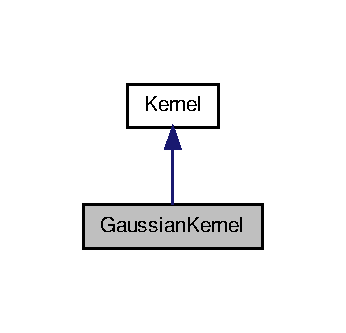
\includegraphics[width=166pt]{classGaussianKernel__inherit__graph}
\end{center}
\end{figure}


\-Collaboration diagram for \-Gaussian\-Kernel\-:
\nopagebreak
\begin{figure}[H]
\begin{center}
\leavevmode
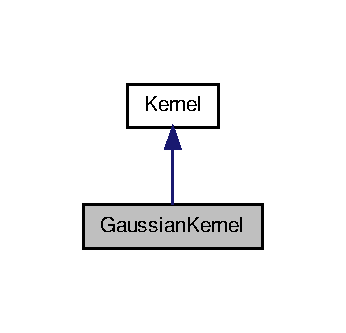
\includegraphics[width=166pt]{classGaussianKernel__coll__graph}
\end{center}
\end{figure}
\subsection*{\-Public \-Member \-Functions}
\begin{DoxyCompactItemize}
\item 
\hypertarget{classGaussianKernel_a35f271df46c73b532d7610c4b374b8d5}{\hyperlink{classGaussianKernel_a35f271df46c73b532d7610c4b374b8d5}{\-Gaussian\-Kernel} (double smoothinglength)}\label{classGaussianKernel_a35f271df46c73b532d7610c4b374b8d5}

\begin{DoxyCompactList}\small\item\em ctor \end{DoxyCompactList}\item 
\hypertarget{classGaussianKernel_a15bac60eda4d2df8bf705457bec9455f}{\hyperlink{classGaussianKernel_a15bac60eda4d2df8bf705457bec9455f}{$\sim$\-Gaussian\-Kernel} ()}\label{classGaussianKernel_a15bac60eda4d2df8bf705457bec9455f}

\begin{DoxyCompactList}\small\item\em dtor \end{DoxyCompactList}\item 
\hypertarget{classGaussianKernel_ae6d613700d1d59f463094cc5c43ce97c}{double \hyperlink{classGaussianKernel_ae6d613700d1d59f463094cc5c43ce97c}{\-W} (double r)}\label{classGaussianKernel_ae6d613700d1d59f463094cc5c43ce97c}

\begin{DoxyCompactList}\small\item\em returns value of \-Gaussian \end{DoxyCompactList}\item 
\hypertarget{classGaussianKernel_a765d88e17749dddc2e3b417f8d74a217}{\hyperlink{structKvector}{\-Kvector} \hyperlink{classGaussianKernel_a765d88e17749dddc2e3b417f8d74a217}{grad\-W} (\hyperlink{structKvector}{\-Kvector} vec1, \hyperlink{structKvector}{\-Kvector} vec2)}\label{classGaussianKernel_a765d88e17749dddc2e3b417f8d74a217}

\begin{DoxyCompactList}\small\item\em returns gradient of \-Gaussian \end{DoxyCompactList}\item 
\hypertarget{classGaussianKernel_ae1233002be9c4d8f814a466056507bc0}{double \hyperlink{classGaussianKernel_ae1233002be9c4d8f814a466056507bc0}{lap\-W} (double r)}\label{classGaussianKernel_ae1233002be9c4d8f814a466056507bc0}

\begin{DoxyCompactList}\small\item\em returns value of the \-Laplacian of \-Gaussian \end{DoxyCompactList}\end{DoxyCompactItemize}


\subsection{\-Detailed \-Description}
\-Gaussian approximation of point particle. 

\-The documentation for this class was generated from the following file\-:\begin{DoxyCompactItemize}
\item 
\hyperlink{gaussiankernel_8h}{gaussiankernel.\-h}\end{DoxyCompactItemize}

\hypertarget{classIncompInvisc}{\section{\-Incomp\-Invisc \-Class \-Reference}
\label{classIncompInvisc}\index{\-Incomp\-Invisc@{\-Incomp\-Invisc}}
}


class for an incompressibe, inviscid fluid  




{\ttfamily \#include $<$incompinvisc.\-h$>$}



\-Inheritance diagram for \-Incomp\-Invisc\-:
\nopagebreak
\begin{figure}[H]
\begin{center}
\leavevmode
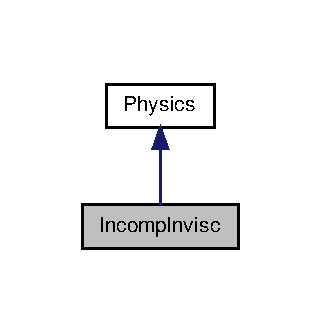
\includegraphics[width=154pt]{classIncompInvisc__inherit__graph}
\end{center}
\end{figure}


\-Collaboration diagram for \-Incomp\-Invisc\-:
\nopagebreak
\begin{figure}[H]
\begin{center}
\leavevmode
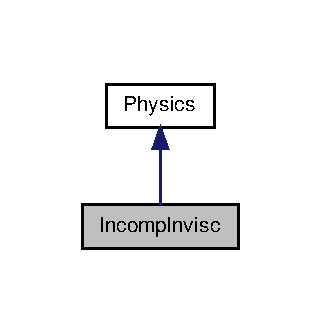
\includegraphics[width=154pt]{classIncompInvisc__coll__graph}
\end{center}
\end{figure}
\subsection*{\-Public \-Member \-Functions}
\begin{DoxyCompactItemize}
\item 
int \hyperlink{classIncompInvisc_a06fbd0a590ef1ef102352a094ae4c698}{rhs} (\hyperlink{classFluid}{\-Fluid} \&fluid, \hyperlink{classParticle}{\-Particle} \&part, \hyperlink{classKernel}{\-Kernel} \&myker, \hyperlink{structProperties}{\-Properties} \&fx)
\begin{DoxyCompactList}\small\item\em update function \end{DoxyCompactList}\item 
\hypertarget{classIncompInvisc_a06483b536f7464b593b55fe4d11a45ce}{int \hyperlink{classIncompInvisc_a06483b536f7464b593b55fe4d11a45ce}{update} (\hyperlink{classParticle}{\-Particle} \&part)}\label{classIncompInvisc_a06483b536f7464b593b55fe4d11a45ce}

\begin{DoxyCompactList}\small\item\em move part's new properties to old properties \end{DoxyCompactList}\item 
\hypertarget{classIncompInvisc_a4363561397ee2a76b67c23851fbaced5}{int \hyperlink{classIncompInvisc_a4363561397ee2a76b67c23851fbaced5}{calc\-Pressure} (\hyperlink{classParticle}{\-Particle} \&part)}\label{classIncompInvisc_a4363561397ee2a76b67c23851fbaced5}

\begin{DoxyCompactList}\small\item\em calculates pressure \end{DoxyCompactList}\item 
\hypertarget{classIncompInvisc_a51217aaa5b957cc843a7a81b59b82518}{int {\bfseries init\-Pressure\-Params} ()}\label{classIncompInvisc_a51217aaa5b957cc843a7a81b59b82518}

\end{DoxyCompactItemize}


\subsection{\-Detailed \-Description}
class for an incompressibe, inviscid fluid 

\subsection{\-Member \-Function \-Documentation}
\hypertarget{classIncompInvisc_a06fbd0a590ef1ef102352a094ae4c698}{\index{\-Incomp\-Invisc@{\-Incomp\-Invisc}!rhs@{rhs}}
\index{rhs@{rhs}!IncompInvisc@{\-Incomp\-Invisc}}
\subsubsection[{rhs}]{\setlength{\rightskip}{0pt plus 5cm}int {\bf \-Incomp\-Invisc\-::rhs} (
\begin{DoxyParamCaption}
\item[{{\bf \-Fluid} \&}]{fluid, }
\item[{{\bf \-Particle} \&}]{part, }
\item[{{\bf \-Kernel} \&}]{myker, }
\item[{{\bf \-Properties} \&}]{fx}
\end{DoxyParamCaption}
)\hspace{0.3cm}{\ttfamily  \mbox{[}virtual\mbox{]}}}}\label{classIncompInvisc_a06fbd0a590ef1ef102352a094ae4c698}


update function 


\begin{DoxyParams}{\-Parameters}
{\em fluid} & input fluid \\
\hline
{\em part} & particular fluid particle \\
\hline
{\em myker} & kernel to use \\
\hline
{\em fx} & stores changes of update \\
\hline
\end{DoxyParams}


\-Implements \hyperlink{classPhysics_a0fd5afe65228da08e3886e58d5285d43}{\-Physics}.



\-The documentation for this class was generated from the following file\-:\begin{DoxyCompactItemize}
\item 
\hyperlink{incompinvisc_8h}{incompinvisc.\-h}\end{DoxyCompactItemize}

\hypertarget{classIncompVisc}{\section{\-Incomp\-Visc \-Class \-Reference}
\label{classIncompVisc}\index{\-Incomp\-Visc@{\-Incomp\-Visc}}
}


class for an incompressible fluid with the inclusion of viscous forces  




{\ttfamily \#include $<$incompvisc.\-h$>$}

\-Inheritance diagram for \-Incomp\-Visc\-:\begin{figure}[H]
\begin{center}
\leavevmode
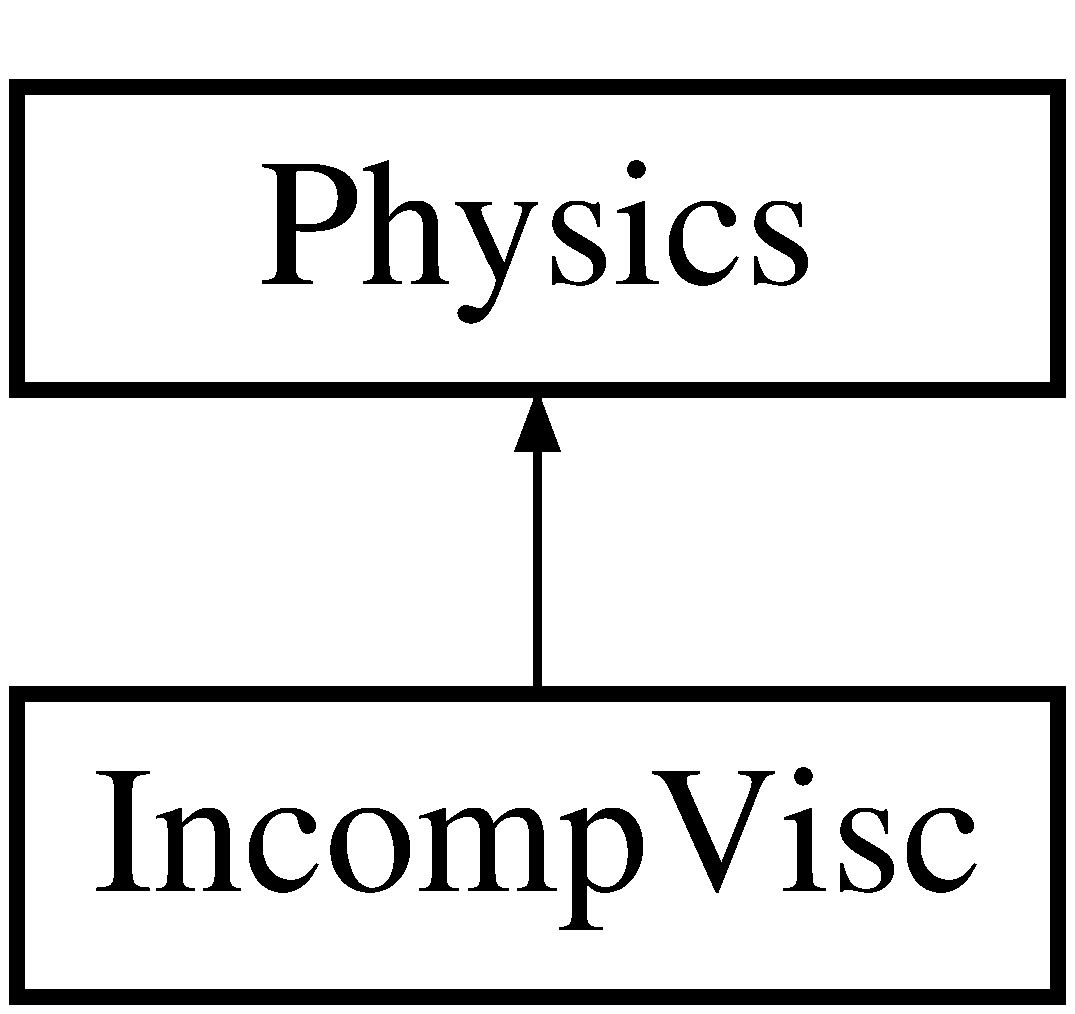
\includegraphics[height=2.000000cm]{classIncompVisc}
\end{center}
\end{figure}
\subsection*{\-Public \-Member \-Functions}
\begin{DoxyCompactItemize}
\item 
\hyperlink{classIncompVisc_a30ec80f360669cb6549710bc6d8b1571}{\-Incomp\-Visc} (double smoothinglength, double grav, double press\-B, double press\-Gamma, double rho\-\_\-0, double visc\-Mu, double visc\-Eta)
\begin{DoxyCompactList}\small\item\em ctor \end{DoxyCompactList}\item 
int \hyperlink{classIncompVisc_a937b901289ff887f072c36b66e9360e8}{rhs} (\hyperlink{classFluid}{\-Fluid} \&fluid, \hyperlink{classParticle}{\-Particle} \&part, \hyperlink{classKernel}{\-Kernel} \&myker, \hyperlink{structProperties}{\-Properties} \&fx)
\begin{DoxyCompactList}\small\item\em update function \end{DoxyCompactList}\item 
\hypertarget{classIncompVisc_a21d2b01dfc8239e08970a94726c016e3}{int \hyperlink{classIncompVisc_a21d2b01dfc8239e08970a94726c016e3}{update} (\hyperlink{classParticle}{\-Particle} \&part)}\label{classIncompVisc_a21d2b01dfc8239e08970a94726c016e3}

\begin{DoxyCompactList}\small\item\em move part's new properties to old properties \end{DoxyCompactList}\item 
\hypertarget{classIncompVisc_a507655c39e5e76e18bd8bd422879984e}{int \hyperlink{classIncompVisc_a507655c39e5e76e18bd8bd422879984e}{calc\-Pressure} (\hyperlink{classParticle}{\-Particle} \&part)}\label{classIncompVisc_a507655c39e5e76e18bd8bd422879984e}

\begin{DoxyCompactList}\small\item\em calculates pressure \end{DoxyCompactList}\item 
\hypertarget{classIncompVisc_a63138bdbcda1877e621027d271848ba6}{int {\bfseries init\-Pressure\-Params} ()}\label{classIncompVisc_a63138bdbcda1877e621027d271848ba6}

\end{DoxyCompactItemize}


\subsection{\-Detailed \-Description}
class for an incompressible fluid with the inclusion of viscous forces 

\subsection{\-Constructor \& \-Destructor \-Documentation}
\hypertarget{classIncompVisc_a30ec80f360669cb6549710bc6d8b1571}{\index{\-Incomp\-Visc@{\-Incomp\-Visc}!\-Incomp\-Visc@{\-Incomp\-Visc}}
\index{\-Incomp\-Visc@{\-Incomp\-Visc}!IncompVisc@{\-Incomp\-Visc}}
\subsubsection[{\-Incomp\-Visc}]{\setlength{\rightskip}{0pt plus 5cm}{\bf \-Incomp\-Visc\-::\-Incomp\-Visc} (
\begin{DoxyParamCaption}
\item[{double}]{smoothinglength, }
\item[{double}]{grav, }
\item[{double}]{press\-B, }
\item[{double}]{press\-Gamma, }
\item[{double}]{rho\-\_\-0, }
\item[{double}]{visc\-Mu, }
\item[{double}]{visc\-Eta}
\end{DoxyParamCaption}
)}}\label{classIncompVisc_a30ec80f360669cb6549710bc6d8b1571}


ctor 


\begin{DoxyParams}{\-Parameters}
{\em smoothinglength} & input smoothinglength of fluid \\
\hline
{\em grav} & input gravitational acceleration \\
\hline
{\em press\-B} & input pressure coefficient \-B \\
\hline
{\em press\-Gamma} & input pressure exponent \-Gamma \\
\hline
{\em rho\-\_\-0} & input reference density \\
\hline
{\em visc\-Mu} & input viscosity parameter mu \\
\hline
{\em visc\-Eta} & inpu tviscosity parameter eta \\
\hline
\end{DoxyParams}


\subsection{\-Member \-Function \-Documentation}
\hypertarget{classIncompVisc_a937b901289ff887f072c36b66e9360e8}{\index{\-Incomp\-Visc@{\-Incomp\-Visc}!rhs@{rhs}}
\index{rhs@{rhs}!IncompVisc@{\-Incomp\-Visc}}
\subsubsection[{rhs}]{\setlength{\rightskip}{0pt plus 5cm}int {\bf \-Incomp\-Visc\-::rhs} (
\begin{DoxyParamCaption}
\item[{{\bf \-Fluid} \&}]{fluid, }
\item[{{\bf \-Particle} \&}]{part, }
\item[{{\bf \-Kernel} \&}]{myker, }
\item[{{\bf \-Properties} \&}]{fx}
\end{DoxyParamCaption}
)\hspace{0.3cm}{\ttfamily  \mbox{[}virtual\mbox{]}}}}\label{classIncompVisc_a937b901289ff887f072c36b66e9360e8}


update function 


\begin{DoxyParams}{\-Parameters}
{\em fluid} & input fluid \\
\hline
{\em part} & particular fluid particle \\
\hline
{\em myker} & kernel to use \\
\hline
{\em fx} & stores changes of update \\
\hline
\end{DoxyParams}


\-Implements \hyperlink{classPhysics_a0fd5afe65228da08e3886e58d5285d43}{\-Physics}.



\-The documentation for this class was generated from the following file\-:\begin{DoxyCompactItemize}
\item 
\hyperlink{incompvisc_8h}{incompvisc.\-h}\end{DoxyCompactItemize}

\hypertarget{classIntegrator}{\section{\-Integrator \-Class \-Reference}
\label{classIntegrator}\index{\-Integrator@{\-Integrator}}
}


superclass for integrators  




{\ttfamily \#include $<$integrator.\-h$>$}

\-Inheritance diagram for \-Integrator\-:\begin{figure}[H]
\begin{center}
\leavevmode
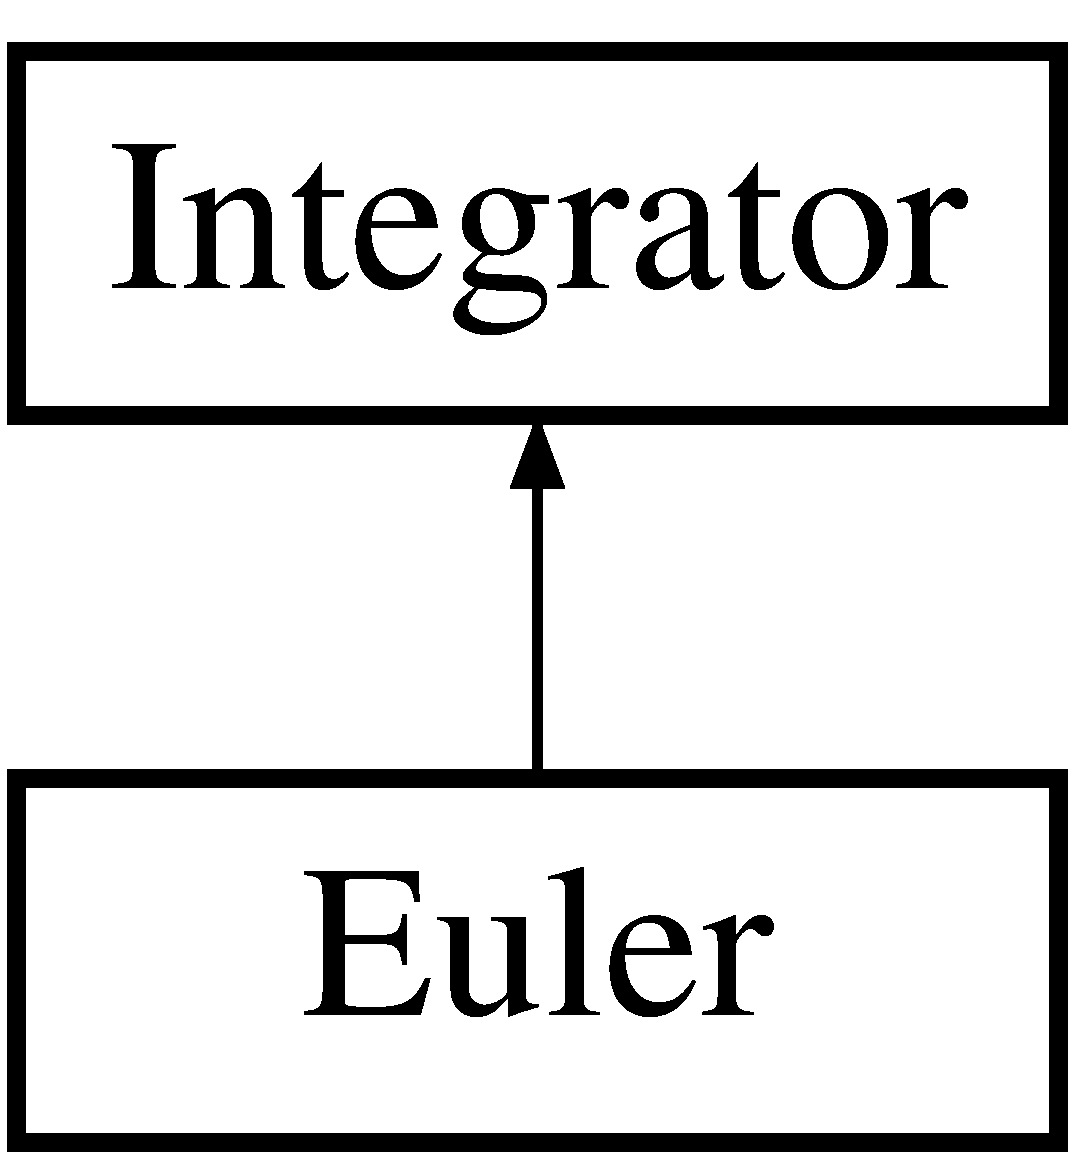
\includegraphics[height=2.000000cm]{classIntegrator}
\end{center}
\end{figure}
\subsection*{\-Public \-Member \-Functions}
\begin{DoxyCompactItemize}
\item 
\hypertarget{classIntegrator_ada0ac381fb6d891c8074fd1ed2102229}{virtual \hyperlink{classIntegrator_ada0ac381fb6d891c8074fd1ed2102229}{$\sim$\-Integrator} ()}\label{classIntegrator_ada0ac381fb6d891c8074fd1ed2102229}

\begin{DoxyCompactList}\small\item\em dtor \end{DoxyCompactList}\item 
\hypertarget{classIntegrator_a453bb8d88d3e35e6212bb43d61ef7253}{virtual int \hyperlink{classIntegrator_a453bb8d88d3e35e6212bb43d61ef7253}{step} ()=0}\label{classIntegrator_a453bb8d88d3e35e6212bb43d61ef7253}

\begin{DoxyCompactList}\small\item\em required function advancing one timestep \end{DoxyCompactList}\end{DoxyCompactItemize}


\subsection{\-Detailed \-Description}
superclass for integrators 

\-The documentation for this class was generated from the following file\-:\begin{DoxyCompactItemize}
\item 
\hyperlink{integrator_8h}{integrator.\-h}\end{DoxyCompactItemize}

\hypertarget{classKernel}{\section{\-Kernel \-Class \-Reference}
\label{classKernel}\index{\-Kernel@{\-Kernel}}
}


smooth kernels approximating point particles  




{\ttfamily \#include $<$kernel.\-h$>$}



\-Inheritance diagram for \-Kernel\-:\nopagebreak
\begin{figure}[H]
\begin{center}
\leavevmode
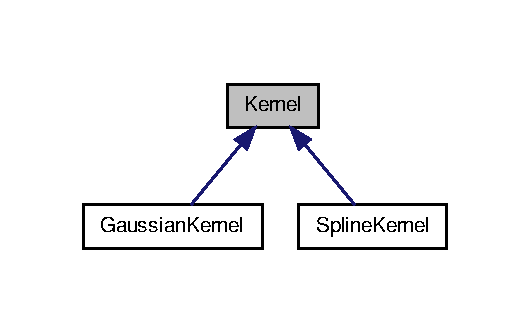
\includegraphics[width=254pt]{classKernel__inherit__graph}
\end{center}
\end{figure}
\subsection*{\-Public \-Member \-Functions}
\begin{DoxyCompactItemize}
\item 
\hypertarget{classKernel_ab0aee98e27b5f821688faad456185b43}{virtual \hyperlink{classKernel_ab0aee98e27b5f821688faad456185b43}{$\sim$\-Kernel} ()}\label{classKernel_ab0aee98e27b5f821688faad456185b43}

\begin{DoxyCompactList}\small\item\em ctor \end{DoxyCompactList}\item 
\hypertarget{classKernel_abdb6d8bdaf6f167019425a067d49bf19}{virtual double \hyperlink{classKernel_abdb6d8bdaf6f167019425a067d49bf19}{\-W} (double r)=0}\label{classKernel_abdb6d8bdaf6f167019425a067d49bf19}

\begin{DoxyCompactList}\small\item\em returns value of kernel function \end{DoxyCompactList}\item 
\hypertarget{classKernel_ae252a58c618b333516e38e780aa9eb04}{virtual \hyperlink{structKvector}{\-Kvector} \hyperlink{classKernel_ae252a58c618b333516e38e780aa9eb04}{grad\-W} (\hyperlink{structKvector}{\-Kvector} vec1, \hyperlink{structKvector}{\-Kvector} vec2)=0}\label{classKernel_ae252a58c618b333516e38e780aa9eb04}

\begin{DoxyCompactList}\small\item\em returns gradient of kernel function \end{DoxyCompactList}\item 
\hypertarget{classKernel_ad2adf6c83967929de6a3f4a6911554c2}{virtual double \hyperlink{classKernel_ad2adf6c83967929de6a3f4a6911554c2}{lap\-W} (double r)=0}\label{classKernel_ad2adf6c83967929de6a3f4a6911554c2}

\begin{DoxyCompactList}\small\item\em returns value of the laplacian of the kernel function \end{DoxyCompactList}\end{DoxyCompactItemize}


\subsection{\-Detailed \-Description}
smooth kernels approximating point particles 

\-The documentation for this class was generated from the following file\-:\begin{DoxyCompactItemize}
\item 
\hyperlink{kernel_8h}{kernel.\-h}\end{DoxyCompactItemize}

\hypertarget{structKvector}{\section{\-Kvector \-Struct \-Reference}
\label{structKvector}\index{\-Kvector@{\-Kvector}}
}


struct for 2\-D vector useful for kernel operations  




{\ttfamily \#include $<$kvector.\-h$>$}

\subsection*{\-Public \-Attributes}
\begin{DoxyCompactItemize}
\item 
\hypertarget{structKvector_ab60dcfd33341d908dcad2306bd11e3e3}{double {\bfseries x}}\label{structKvector_ab60dcfd33341d908dcad2306bd11e3e3}

\item 
\hypertarget{structKvector_a56d7ba00fc9d34e15f5c1e391bf466f4}{double {\bfseries y}}\label{structKvector_a56d7ba00fc9d34e15f5c1e391bf466f4}

\end{DoxyCompactItemize}


\subsection{\-Detailed \-Description}
struct for 2\-D vector useful for kernel operations 

\-The documentation for this struct was generated from the following file\-:\begin{DoxyCompactItemize}
\item 
\hyperlink{kvector_8h}{kvector.\-h}\end{DoxyCompactItemize}

\hypertarget{classOutput}{\section{\-Output \-Class \-Reference}
\label{classOutput}\index{\-Output@{\-Output}}
}


\-Class to build output file for fluid state.  




{\ttfamily \#include $<$output.\-h$>$}

\subsection*{\-Public \-Member \-Functions}
\begin{DoxyCompactItemize}
\item 
\hypertarget{classOutput_a80fc4c990bded1578523fb41f50c7079}{\hyperlink{classOutput_a80fc4c990bded1578523fb41f50c7079}{\-Output} (const std\-::string \&filename)}\label{classOutput_a80fc4c990bded1578523fb41f50c7079}

\begin{DoxyCompactList}\small\item\em create file to hold fluid properties \end{DoxyCompactList}\item 
void \hyperlink{classOutput_ad00a1d373d263c97e538156d9802a7da}{write} (double t, const \hyperlink{classFluid}{\-Fluid} \&fluid)
\begin{DoxyCompactList}\small\item\em write fluid properties \end{DoxyCompactList}\end{DoxyCompactItemize}


\subsection{\-Detailed \-Description}
\-Class to build output file for fluid state. 

\subsection{\-Member \-Function \-Documentation}
\hypertarget{classOutput_ad00a1d373d263c97e538156d9802a7da}{\index{\-Output@{\-Output}!write@{write}}
\index{write@{write}!Output@{\-Output}}
\subsubsection[{write}]{\setlength{\rightskip}{0pt plus 5cm}void {\bf \-Output\-::write} (
\begin{DoxyParamCaption}
\item[{double}]{t, }
\item[{const {\bf \-Fluid} \&}]{fluid}
\end{DoxyParamCaption}
)}}\label{classOutput_ad00a1d373d263c97e538156d9802a7da}


write fluid properties 

fluid 
\begin{DoxyParams}{\-Parameters}
{\em t} & current time \\
\hline
\end{DoxyParams}


\-The documentation for this class was generated from the following file\-:\begin{DoxyCompactItemize}
\item 
\hyperlink{output_8h}{output.\-h}\end{DoxyCompactItemize}

\hypertarget{classParticle}{\section{\-Particle \-Class \-Reference}
\label{classParticle}\index{\-Particle@{\-Particle}}
}


\hyperlink{structProperties}{\-Properties} and functions for individual particles.  




{\ttfamily \#include $<$particle.\-h$>$}

\subsection*{\-Public \-Types}
\begin{DoxyCompactItemize}
\item 
\hypertarget{classParticle_aded94129b877208bb64f1af2c51742d1}{typedef int {\bfseries \-Tag}}\label{classParticle_aded94129b877208bb64f1af2c51742d1}

\item 
\hypertarget{classParticle_a0724b5e0276679c358b729a26f9629a4}{typedef std\-::vector$<$ int $>$ {\bfseries \-Tag\-Array}}\label{classParticle_a0724b5e0276679c358b729a26f9629a4}

\end{DoxyCompactItemize}
\subsection*{\-Public \-Member \-Functions}
\begin{DoxyCompactItemize}
\item 
\hypertarget{classParticle_a88358bdce88d9dda12e57c5ff976dca5}{\hyperlink{classParticle_a88358bdce88d9dda12e57c5ff976dca5}{\-Particle} (\-Tag tag, size\-\_\-t \-N, size\-\_\-t \-N\-B, const \hyperlink{structProperties}{\-Properties} \&properties)}\label{classParticle_a88358bdce88d9dda12e57c5ff976dca5}

\begin{DoxyCompactList}\small\item\em ctor \end{DoxyCompactList}\item 
\hypertarget{classParticle_ac2bd006400deb1c9f17ddce9d70d3728}{\hyperlink{structProperties}{\-Properties} \hyperlink{classParticle_ac2bd006400deb1c9f17ddce9d70d3728}{get\-Old\-Properties} () const }\label{classParticle_ac2bd006400deb1c9f17ddce9d70d3728}

\begin{DoxyCompactList}\small\item\em return old version of particle properties \end{DoxyCompactList}\item 
\hypertarget{classParticle_a4dd65686cc2494434cab8db8a2a8e923}{\hyperlink{structProperties}{\-Properties} \hyperlink{classParticle_a4dd65686cc2494434cab8db8a2a8e923}{get\-New\-Properties} () const }\label{classParticle_a4dd65686cc2494434cab8db8a2a8e923}

\begin{DoxyCompactList}\small\item\em return new version of particle properties \end{DoxyCompactList}\item 
\hypertarget{classParticle_a0b1b6f1166d06dbe1ab143c6561bb9cc}{void \hyperlink{classParticle_a0b1b6f1166d06dbe1ab143c6561bb9cc}{set\-Old\-Properties} (const \hyperlink{structProperties}{\-Properties} \&props)}\label{classParticle_a0b1b6f1166d06dbe1ab143c6561bb9cc}

\begin{DoxyCompactList}\small\item\em set old version of particle properties \end{DoxyCompactList}\item 
\hypertarget{classParticle_afea2eefc83b471a45c9b1e6c442b91c6}{void \hyperlink{classParticle_afea2eefc83b471a45c9b1e6c442b91c6}{set\-New\-Properties} (const \hyperlink{structProperties}{\-Properties} \&props)}\label{classParticle_afea2eefc83b471a45c9b1e6c442b91c6}

\begin{DoxyCompactList}\small\item\em set new version of particle properties \end{DoxyCompactList}\item 
\hypertarget{classParticle_a3ac6511d98e8472de59bb474dfe851a1}{void \hyperlink{classParticle_a3ac6511d98e8472de59bb474dfe851a1}{add\-Neighbor} (const \hyperlink{classParticle}{\-Particle} \&neighbor)}\label{classParticle_a3ac6511d98e8472de59bb474dfe851a1}

\begin{DoxyCompactList}\small\item\em add a neighbor tag \end{DoxyCompactList}\item 
\hypertarget{classParticle_a19bc575957444c91ed5c236e065673ac}{void \hyperlink{classParticle_a19bc575957444c91ed5c236e065673ac}{add\-Boundary\-Neighbor} (const \hyperlink{classParticle}{\-Particle} \&neighbor)}\label{classParticle_a19bc575957444c91ed5c236e065673ac}

\begin{DoxyCompactList}\small\item\em add a boundary neighbor tag \end{DoxyCompactList}\item 
\hypertarget{classParticle_addaece13cd072de3db9b3281262a9793}{size\-\_\-t \hyperlink{classParticle_addaece13cd072de3db9b3281262a9793}{number\-Of\-Neighbors} () const }\label{classParticle_addaece13cd072de3db9b3281262a9793}

\begin{DoxyCompactList}\small\item\em return the number of neighbors (neighbors\-\_\-) \end{DoxyCompactList}\item 
\hypertarget{classParticle_a73a8242d6ee30d116ca6bdf952bd7b89}{size\-\_\-t \hyperlink{classParticle_a73a8242d6ee30d116ca6bdf952bd7b89}{number\-Of\-Boundary\-Neighbors} () const }\label{classParticle_a73a8242d6ee30d116ca6bdf952bd7b89}

\begin{DoxyCompactList}\small\item\em return the number of boundary neighbors (boundaryneighbors\-\_\-) \end{DoxyCompactList}\item 
\hypertarget{classParticle_ae3e4f71b6d03c5e100674e8dead0565e}{\-Tag\-Array \hyperlink{classParticle_ae3e4f71b6d03c5e100674e8dead0565e}{get\-Neighbors} () const }\label{classParticle_ae3e4f71b6d03c5e100674e8dead0565e}

\begin{DoxyCompactList}\small\item\em return the array of neighbor tags (neighborarray\-\_\-) \end{DoxyCompactList}\item 
\hypertarget{classParticle_a13ece3496e8e2510d7302d1692b5090d}{\-Tag\-Array \hyperlink{classParticle_a13ece3496e8e2510d7302d1692b5090d}{get\-Boundary\-Neighbors} () const }\label{classParticle_a13ece3496e8e2510d7302d1692b5090d}

\begin{DoxyCompactList}\small\item\em return the array of boundary neighbor tags (boundaryneighborarray\-\_\-) \end{DoxyCompactList}\item 
\hypertarget{classParticle_adce0a40cce7f7862ff2fc0e6bab2e3f4}{\-Tag \hyperlink{classParticle_adce0a40cce7f7862ff2fc0e6bab2e3f4}{get\-Tag} () const }\label{classParticle_adce0a40cce7f7862ff2fc0e6bab2e3f4}

\begin{DoxyCompactList}\small\item\em return the particle's tag (tag\-\_\-) \end{DoxyCompactList}\item 
\hypertarget{classParticle_a54b1e463538ca132ca86c758ca1f04c2}{void \hyperlink{classParticle_a54b1e463538ca132ca86c758ca1f04c2}{delete\-Neighbors} ()}\label{classParticle_a54b1e463538ca132ca86c758ca1f04c2}

\begin{DoxyCompactList}\small\item\em re-\/initiliaze neighborarray\-\_\- and boundaryneighborarray\-\_\- \end{DoxyCompactList}\end{DoxyCompactItemize}


\subsection{\-Detailed \-Description}
\hyperlink{structProperties}{\-Properties} and functions for individual particles. 

\-The documentation for this class was generated from the following file\-:\begin{DoxyCompactItemize}
\item 
\hyperlink{particle_8h}{particle.\-h}\end{DoxyCompactItemize}

\hypertarget{classPhysics}{\section{\-Physics \-Class \-Reference}
\label{classPhysics}\index{\-Physics@{\-Physics}}
}


superclass for implementing different fluid physics  




{\ttfamily \#include $<$physics.\-h$>$}



\-Inheritance diagram for \-Physics\-:
\nopagebreak
\begin{figure}[H]
\begin{center}
\leavevmode
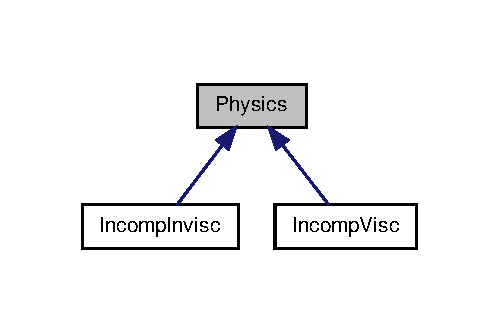
\includegraphics[width=240pt]{classPhysics__inherit__graph}
\end{center}
\end{figure}
\subsection*{\-Public \-Member \-Functions}
\begin{DoxyCompactItemize}
\item 
\hypertarget{classPhysics_afdd87b5bb9fe2e927c37d50fbeb8216b}{virtual \hyperlink{classPhysics_afdd87b5bb9fe2e927c37d50fbeb8216b}{$\sim$\-Physics} ()}\label{classPhysics_afdd87b5bb9fe2e927c37d50fbeb8216b}

\begin{DoxyCompactList}\small\item\em dtor \end{DoxyCompactList}\item 
virtual int \hyperlink{classPhysics_a0fd5afe65228da08e3886e58d5285d43}{rhs} (\hyperlink{classFluid}{\-Fluid} \&fluid, \hyperlink{classParticle}{\-Particle} \&part, \hyperlink{classKernel}{\-Kernel} \&my\-Ker, \hyperlink{structProperties}{\-Properties} \&fx)=0
\begin{DoxyCompactList}\small\item\em update function \end{DoxyCompactList}\item 
\hypertarget{classPhysics_ab51a11d51e09b132610cd6fbb95d0c0c}{virtual int \hyperlink{classPhysics_ab51a11d51e09b132610cd6fbb95d0c0c}{update} (\hyperlink{classParticle}{\-Particle} \&part)=0}\label{classPhysics_ab51a11d51e09b132610cd6fbb95d0c0c}

\begin{DoxyCompactList}\small\item\em move part's new properties to old properties \end{DoxyCompactList}\item 
\hypertarget{classPhysics_a50759e0407dff12021c94f9fa6729765}{virtual int \hyperlink{classPhysics_a50759e0407dff12021c94f9fa6729765}{calc\-Pressure} (\hyperlink{classParticle}{\-Particle} \&part)=0}\label{classPhysics_a50759e0407dff12021c94f9fa6729765}

\begin{DoxyCompactList}\small\item\em calculates pressure \end{DoxyCompactList}\item 
\hypertarget{classPhysics_a933c3288d21bd8dbdab422d4fe09f84d}{virtual int {\bfseries init\-Pressure\-Params} ()=0}\label{classPhysics_a933c3288d21bd8dbdab422d4fe09f84d}

\end{DoxyCompactItemize}


\subsection{\-Detailed \-Description}
superclass for implementing different fluid physics 

\subsection{\-Member \-Function \-Documentation}
\hypertarget{classPhysics_a0fd5afe65228da08e3886e58d5285d43}{\index{\-Physics@{\-Physics}!rhs@{rhs}}
\index{rhs@{rhs}!Physics@{\-Physics}}
\subsubsection[{rhs}]{\setlength{\rightskip}{0pt plus 5cm}virtual int {\bf \-Physics\-::rhs} (
\begin{DoxyParamCaption}
\item[{{\bf \-Fluid} \&}]{fluid, }
\item[{{\bf \-Particle} \&}]{part, }
\item[{{\bf \-Kernel} \&}]{my\-Ker, }
\item[{{\bf \-Properties} \&}]{fx}
\end{DoxyParamCaption}
)\hspace{0.3cm}{\ttfamily  \mbox{[}pure virtual\mbox{]}}}}\label{classPhysics_a0fd5afe65228da08e3886e58d5285d43}


update function 


\begin{DoxyParams}{\-Parameters}
{\em fluid} & input fluid \\
\hline
{\em part} & particular fluid particle \\
\hline
{\em my\-Ker} & kernel to use \\
\hline
{\em fx} & stores changes of update \\
\hline
\end{DoxyParams}


\-Implemented in \hyperlink{classIncompVisc_a937b901289ff887f072c36b66e9360e8}{\-Incomp\-Visc}, and \hyperlink{classIncompInvisc_a06fbd0a590ef1ef102352a094ae4c698}{\-Incomp\-Invisc}.



\-The documentation for this class was generated from the following file\-:\begin{DoxyCompactItemize}
\item 
\hyperlink{physics_8h}{physics.\-h}\end{DoxyCompactItemize}

\hypertarget{classPredictorCorrector}{\section{\-Predictor\-Corrector \-Class \-Reference}
\label{classPredictorCorrector}\index{\-Predictor\-Corrector@{\-Predictor\-Corrector}}
}


\-Predictor-\/corrector integrator.  




{\ttfamily \#include $<$predictorcorrector.\-h$>$}



\-Inheritance diagram for \-Predictor\-Corrector\-:
\nopagebreak
\begin{figure}[H]
\begin{center}
\leavevmode
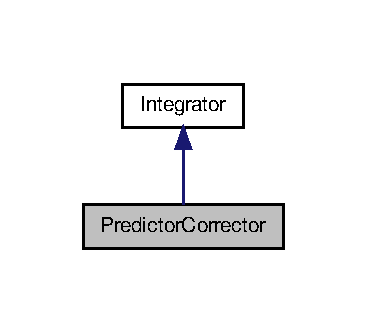
\includegraphics[width=176pt]{classPredictorCorrector__inherit__graph}
\end{center}
\end{figure}


\-Collaboration diagram for \-Predictor\-Corrector\-:
\nopagebreak
\begin{figure}[H]
\begin{center}
\leavevmode
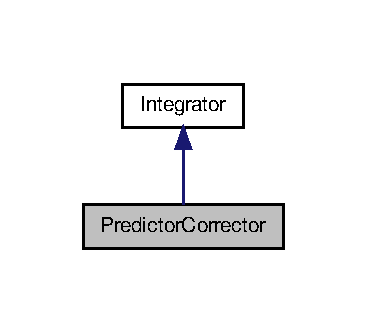
\includegraphics[width=176pt]{classPredictorCorrector__coll__graph}
\end{center}
\end{figure}
\subsection*{\-Public \-Member \-Functions}
\begin{DoxyCompactItemize}
\item 
\hypertarget{classPredictorCorrector_ad39d1bbacf7a674d630a44ec67c6e2c0}{\hyperlink{classPredictorCorrector_ad39d1bbacf7a674d630a44ec67c6e2c0}{\-Predictor\-Corrector} (double dt, \hyperlink{classFluid}{\-Fluid} \&fluid, \hyperlink{classPhysics}{\-Physics} \&physics)}\label{classPredictorCorrector_ad39d1bbacf7a674d630a44ec67c6e2c0}

\begin{DoxyCompactList}\small\item\em ctor \end{DoxyCompactList}\item 
\hypertarget{classPredictorCorrector_aec41b3501a2d94a04e74395f9877ad6f}{int \hyperlink{classPredictorCorrector_aec41b3501a2d94a04e74395f9877ad6f}{step} ()}\label{classPredictorCorrector_aec41b3501a2d94a04e74395f9877ad6f}

\begin{DoxyCompactList}\small\item\em advances one timestep \end{DoxyCompactList}\end{DoxyCompactItemize}


\subsection{\-Detailed \-Description}
\-Predictor-\/corrector integrator. 

\-The documentation for this class was generated from the following file\-:\begin{DoxyCompactItemize}
\item 
\hyperlink{predictorcorrector_8h}{predictorcorrector.\-h}\end{DoxyCompactItemize}

\hypertarget{structProperties}{\section{\-Properties \-Struct \-Reference}
\label{structProperties}\index{\-Properties@{\-Properties}}
}


struct holding physical particle properties  




{\ttfamily \#include $<$properties.\-h$>$}

\subsection*{\-Public \-Attributes}
\begin{DoxyCompactItemize}
\item 
\hypertarget{structProperties_a2e6b709c527c9206db00891ad1b83240}{double \hyperlink{structProperties_a2e6b709c527c9206db00891ad1b83240}{x}}\label{structProperties_a2e6b709c527c9206db00891ad1b83240}

\begin{DoxyCompactList}\small\item\em x position \end{DoxyCompactList}\item 
\hypertarget{structProperties_a3a6af08782493b20c894f1a68311b54e}{double \hyperlink{structProperties_a3a6af08782493b20c894f1a68311b54e}{y}}\label{structProperties_a3a6af08782493b20c894f1a68311b54e}

\begin{DoxyCompactList}\small\item\em y position \end{DoxyCompactList}\item 
\hypertarget{structProperties_abc41eaad5d918caa22d09be4fe7e6982}{double \hyperlink{structProperties_abc41eaad5d918caa22d09be4fe7e6982}{u}}\label{structProperties_abc41eaad5d918caa22d09be4fe7e6982}

\begin{DoxyCompactList}\small\item\em x velocity \end{DoxyCompactList}\item 
\hypertarget{structProperties_a1598f451b61d5066887bbe4ed8db07a1}{double \hyperlink{structProperties_a1598f451b61d5066887bbe4ed8db07a1}{v}}\label{structProperties_a1598f451b61d5066887bbe4ed8db07a1}

\begin{DoxyCompactList}\small\item\em y velocity \end{DoxyCompactList}\item 
\hypertarget{structProperties_a8ae0297de69be0dae8b291d9716d68a4}{double \hyperlink{structProperties_a8ae0297de69be0dae8b291d9716d68a4}{density}}\label{structProperties_a8ae0297de69be0dae8b291d9716d68a4}

\begin{DoxyCompactList}\small\item\em density at particle \end{DoxyCompactList}\item 
\hypertarget{structProperties_aded5ddc676b930dfbdfa81f78ef2547e}{double \hyperlink{structProperties_aded5ddc676b930dfbdfa81f78ef2547e}{mass}}\label{structProperties_aded5ddc676b930dfbdfa81f78ef2547e}

\begin{DoxyCompactList}\small\item\em particle mass \end{DoxyCompactList}\item 
\hypertarget{structProperties_a001e790a070fc788d99ab472330e70fb}{double \hyperlink{structProperties_a001e790a070fc788d99ab472330e70fb}{pressure}}\label{structProperties_a001e790a070fc788d99ab472330e70fb}

\begin{DoxyCompactList}\small\item\em pressure at particle \end{DoxyCompactList}\item 
\hypertarget{structProperties_a7c07daf004e24ec22e6a12febef4db6f}{double \hyperlink{structProperties_a7c07daf004e24ec22e6a12febef4db6f}{visc}}\label{structProperties_a7c07daf004e24ec22e6a12febef4db6f}

\begin{DoxyCompactList}\small\item\em particle viscosity \end{DoxyCompactList}\end{DoxyCompactItemize}


\subsection{\-Detailed \-Description}
struct holding physical particle properties 

\-The documentation for this struct was generated from the following file\-:\begin{DoxyCompactItemize}
\item 
\hyperlink{properties_8h}{properties.\-h}\end{DoxyCompactItemize}

\hypertarget{classSplineKernel}{\section{\-Spline\-Kernel \-Class \-Reference}
\label{classSplineKernel}\index{\-Spline\-Kernel@{\-Spline\-Kernel}}
}


cubic spline approximation of point particle  




{\ttfamily \#include $<$splinekernel.\-h$>$}

\-Inheritance diagram for \-Spline\-Kernel\-:\begin{figure}[H]
\begin{center}
\leavevmode
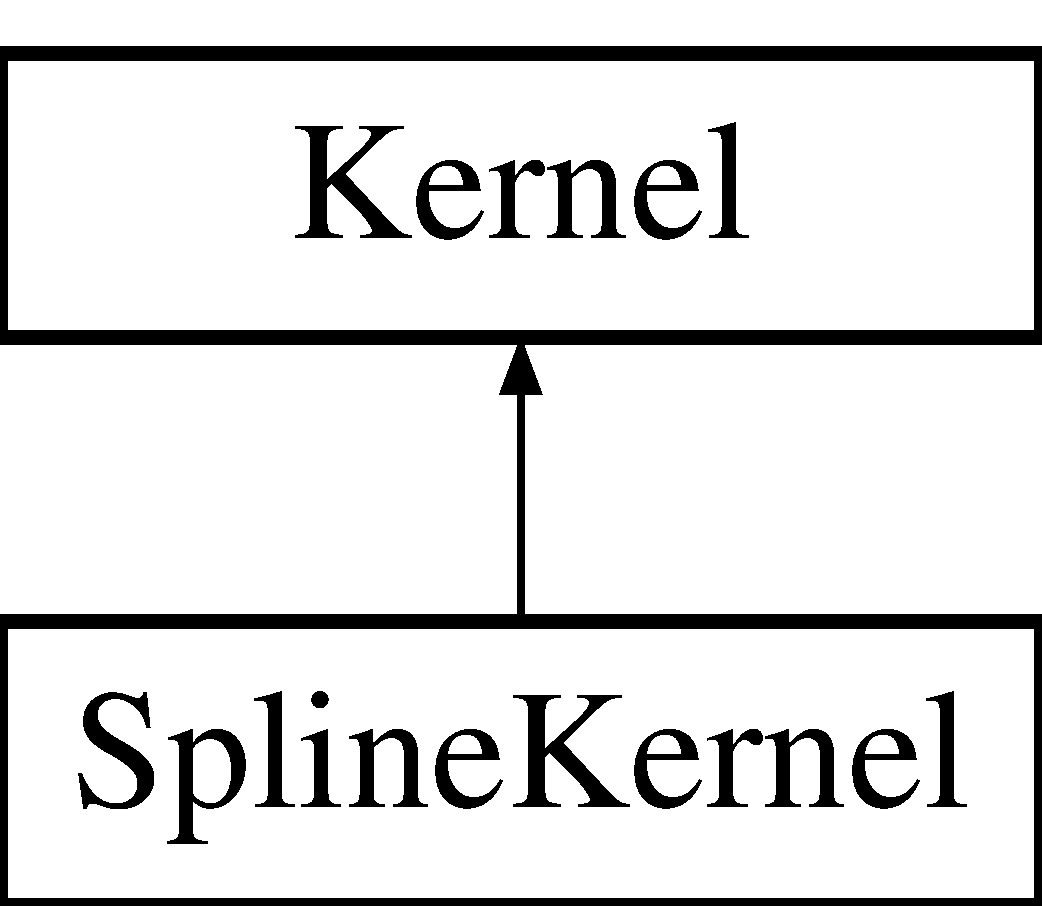
\includegraphics[height=2.000000cm]{classSplineKernel}
\end{center}
\end{figure}
\subsection*{\-Public \-Member \-Functions}
\begin{DoxyCompactItemize}
\item 
\hypertarget{classSplineKernel_a5b2e456001025775c0912f43d5fae88c}{\hyperlink{classSplineKernel_a5b2e456001025775c0912f43d5fae88c}{\-Spline\-Kernel} (double smoothinglength)}\label{classSplineKernel_a5b2e456001025775c0912f43d5fae88c}

\begin{DoxyCompactList}\small\item\em ctor \end{DoxyCompactList}\item 
\hypertarget{classSplineKernel_ab88c7d460702f581c87817c82fe792d2}{\hyperlink{classSplineKernel_ab88c7d460702f581c87817c82fe792d2}{$\sim$\-Spline\-Kernel} ()}\label{classSplineKernel_ab88c7d460702f581c87817c82fe792d2}

\begin{DoxyCompactList}\small\item\em dtor \end{DoxyCompactList}\item 
\hypertarget{classSplineKernel_a8dd3d968b0436c799789da0777398151}{double \hyperlink{classSplineKernel_a8dd3d968b0436c799789da0777398151}{\-W} (double r)}\label{classSplineKernel_a8dd3d968b0436c799789da0777398151}

\begin{DoxyCompactList}\small\item\em returns value of cubic spline \end{DoxyCompactList}\item 
\hypertarget{classSplineKernel_a67e539f362309f2c196a186e565da62b}{\hyperlink{structKvector}{\-Kvector} \hyperlink{classSplineKernel_a67e539f362309f2c196a186e565da62b}{grad\-W} (\hyperlink{structKvector}{\-Kvector} vec1, \hyperlink{structKvector}{\-Kvector} vec2)}\label{classSplineKernel_a67e539f362309f2c196a186e565da62b}

\begin{DoxyCompactList}\small\item\em returns gradient of cubic spline \end{DoxyCompactList}\item 
\hypertarget{classSplineKernel_a51a02339e02aa47138e8a4b0e5bed5cc}{double \hyperlink{classSplineKernel_a51a02339e02aa47138e8a4b0e5bed5cc}{lap\-W} (double r)}\label{classSplineKernel_a51a02339e02aa47138e8a4b0e5bed5cc}

\begin{DoxyCompactList}\small\item\em returns \-Laplacian of cubic spline \end{DoxyCompactList}\end{DoxyCompactItemize}


\subsection{\-Detailed \-Description}
cubic spline approximation of point particle 

\-The documentation for this class was generated from the following file\-:\begin{DoxyCompactItemize}
\item 
\hyperlink{splinekernel_8h}{splinekernel.\-h}\end{DoxyCompactItemize}

\chapter{\-File \-Documentation}
\hypertarget{euler_8h}{\section{euler.\-h \-File \-Reference}
\label{euler_8h}\index{euler.\-h@{euler.\-h}}
}


implementation of euler integrator  


{\ttfamily \#include \char`\"{}integrator.\-h\char`\"{}}\*
\subsection*{\-Classes}
\begin{DoxyCompactItemize}
\item 
class \hyperlink{classEuler}{\-Euler}
\begin{DoxyCompactList}\small\item\em euler integrator \end{DoxyCompactList}\end{DoxyCompactItemize}


\subsection{\-Detailed \-Description}
implementation of euler integrator 
\hypertarget{eulermod_8h}{\section{eulermod.\-h \-File \-Reference}
\label{eulermod_8h}\index{eulermod.\-h@{eulermod.\-h}}
}


implementation of \hyperlink{classEuler}{\-Euler} \hyperlink{classIntegrator}{\-Integrator}, modified so that the position is updated using the updated velocity  


{\ttfamily \#include \char`\"{}integrator.\-h\char`\"{}}\*
{\ttfamily \#include \char`\"{}fluid.\-h\char`\"{}}\*
{\ttfamily \#include \char`\"{}physics.\-h\char`\"{}}\*
{\ttfamily \#include \char`\"{}particle.\-h\char`\"{}}\*
\-Include dependency graph for eulermod.\-h\-:\nopagebreak
\begin{figure}[H]
\begin{center}
\leavevmode
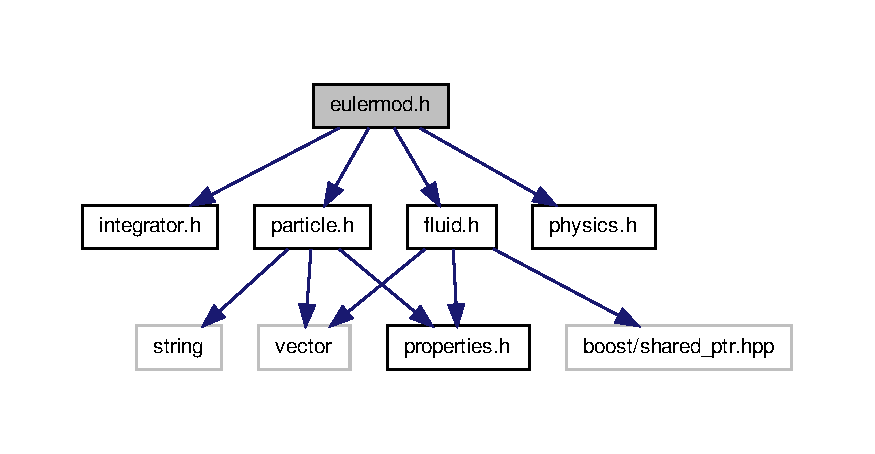
\includegraphics[width=350pt]{eulermod_8h__incl}
\end{center}
\end{figure}
\-This graph shows which files directly or indirectly include this file\-:\nopagebreak
\begin{figure}[H]
\begin{center}
\leavevmode
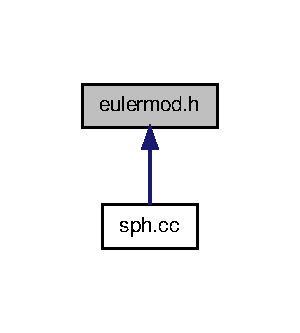
\includegraphics[width=144pt]{eulermod_8h__dep__incl}
\end{center}
\end{figure}
\subsection*{\-Classes}
\begin{DoxyCompactItemize}
\item 
class \hyperlink{classEulermod}{\-Eulermod}
\begin{DoxyCompactList}\small\item\em modified \hyperlink{classEuler}{\-Euler} integrator \end{DoxyCompactList}\end{DoxyCompactItemize}


\subsection{\-Detailed \-Description}
implementation of \hyperlink{classEuler}{\-Euler} \hyperlink{classIntegrator}{\-Integrator}, modified so that the position is updated using the updated velocity 
\hypertarget{fluid_8h}{\section{fluid.\-h \-File \-Reference}
\label{fluid_8h}\index{fluid.\-h@{fluid.\-h}}
}


\-Definition of fluid class for packaging together particles, boundary particles, and their properties.  


{\ttfamily \#include $<$vector$>$}\*
{\ttfamily \#include $<$boost/shared\-\_\-ptr.\-hpp$>$}\*
{\ttfamily \#include \char`\"{}properties.\-h\char`\"{}}\*
\-Include dependency graph for fluid.\-h\-:\nopagebreak
\begin{figure}[H]
\begin{center}
\leavevmode
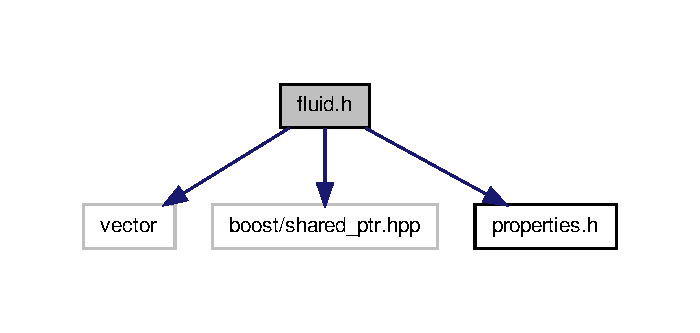
\includegraphics[width=336pt]{fluid_8h__incl}
\end{center}
\end{figure}
\-This graph shows which files directly or indirectly include this file\-:
\nopagebreak
\begin{figure}[H]
\begin{center}
\leavevmode
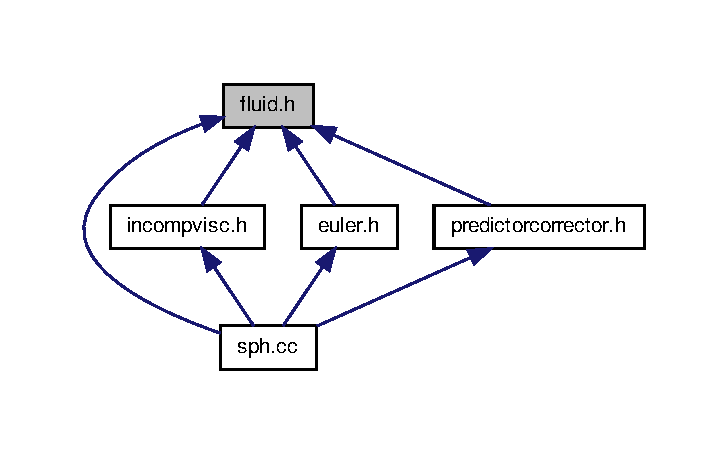
\includegraphics[width=350pt]{fluid_8h__dep__incl}
\end{center}
\end{figure}
\subsection*{\-Classes}
\begin{DoxyCompactItemize}
\item 
class \hyperlink{classFluid}{\-Fluid}
\begin{DoxyCompactList}\small\item\em \-Holds particles and boundary praticles. \end{DoxyCompactList}\end{DoxyCompactItemize}


\subsection{\-Detailed \-Description}
\-Definition of fluid class for packaging together particles, boundary particles, and their properties. 
\hypertarget{fluid__test_8cc}{\section{fluid\-\_\-test.\-cc \-File \-Reference}
\label{fluid__test_8cc}\index{fluid\-\_\-test.\-cc@{fluid\-\_\-test.\-cc}}
}


tests for \hyperlink{classFluid}{\-Fluid}  


{\ttfamily \#include \char`\"{}fluid\-\_\-test.\-h\char`\"{}}\*
\subsection*{\-Functions}
\begin{DoxyCompactItemize}
\item 
\hypertarget{fluid__test_8cc_ade947f733077a049a507b3aa4192133a}{\hyperlink{structProperties}{\-Properties} {\bfseries pos} (double x, double y)}\label{fluid__test_8cc_ade947f733077a049a507b3aa4192133a}

\item 
\hypertarget{fluid__test_8cc_a2f08df650559d3c125c94d4dd1b0aa94}{\hyperlink{fluid__test_8cc_a2f08df650559d3c125c94d4dd1b0aa94}{\-T\-E\-S\-T\-\_\-\-F} (\-Fluid\-Test, check\-Add\-Get\-Boundary)}\label{fluid__test_8cc_a2f08df650559d3c125c94d4dd1b0aa94}

\begin{DoxyCompactList}\small\item\em tests \hyperlink{classFluid_a366795e3ce9fe395ee33febd3813b6f7}{\-Fluid\-::add\-Boundary} and \hyperlink{classFluid_a8c9d7de21e341ec6344e78cb2ca21baf}{\-Fluid\-::get\-Boundaries} \end{DoxyCompactList}\item 
\hypertarget{fluid__test_8cc_a9893813440665bb3bfe040ee8ec857f4}{\hyperlink{fluid__test_8cc_a9893813440665bb3bfe040ee8ec857f4}{\-T\-E\-S\-T\-\_\-\-F} (\-Fluid\-Test, check\-Reset\-Neighbors)}\label{fluid__test_8cc_a9893813440665bb3bfe040ee8ec857f4}

\begin{DoxyCompactList}\small\item\em tests \hyperlink{classFluid_a6f1fc57fb0aa2de6c81134f02c1a82ce}{\-Fluid\-::reset\-Neighbors} undoes neighbor tags \end{DoxyCompactList}\item 
\hypertarget{fluid__test_8cc_a9faac9c71027a5724c134637059dab3c}{\hyperlink{fluid__test_8cc_a9faac9c71027a5724c134637059dab3c}{\-T\-E\-S\-T\-\_\-\-F} (\-Fluid\-Test, check\-Get\-Kernel)}\label{fluid__test_8cc_a9faac9c71027a5724c134637059dab3c}

\begin{DoxyCompactList}\small\item\em tests \hyperlink{classFluid_afb89fa53b31cbd8a053fea20779f7fc0}{\-Fluid\-::get\-Kernel} \end{DoxyCompactList}\item 
\hypertarget{fluid__test_8cc_a63c13289e1951aadfacabcbc19d07b40}{\hyperlink{fluid__test_8cc_a63c13289e1951aadfacabcbc19d07b40}{\-T\-E\-S\-T\-\_\-\-F} (\-Fluid\-Test, check\-Get\-N\-Particles)}\label{fluid__test_8cc_a63c13289e1951aadfacabcbc19d07b40}

\begin{DoxyCompactList}\small\item\em tests \hyperlink{classFluid_a01a17b69aaea73239a3f13f191dbd48a}{\-Fluid\-::get\-N\-Particles} \end{DoxyCompactList}\item 
\hypertarget{fluid__test_8cc_a18d0de37508cbb86613a64e3d78f6166}{\hyperlink{fluid__test_8cc_a18d0de37508cbb86613a64e3d78f6166}{\-T\-E\-S\-T\-\_\-\-F} (\-Fluid\-Test, check\-Get\-N\-Boundaries)}\label{fluid__test_8cc_a18d0de37508cbb86613a64e3d78f6166}

\begin{DoxyCompactList}\small\item\em tests \hyperlink{classFluid_aad2f8ee1598445f42f41e7faf1fd9a09}{\-Fluid\-::get\-N\-Boundaries} \end{DoxyCompactList}\item 
\hypertarget{fluid__test_8cc_af3afea28f5de400cd3d9fcb28d92d022}{\hyperlink{fluid__test_8cc_af3afea28f5de400cd3d9fcb28d92d022}{\-T\-E\-S\-T\-\_\-\-F} (\-Fluid\-Test, check\-Reset\-Particles)}\label{fluid__test_8cc_af3afea28f5de400cd3d9fcb28d92d022}

\begin{DoxyCompactList}\small\item\em tests \hyperlink{classFluid_a1f422a0a94dc16192650ea11db416576}{\-Fluid\-::reset\-Particles} updates particle properties \end{DoxyCompactList}\item 
\hypertarget{fluid__test_8cc_a5fa3c9e3c0d9ed51cf816efdc5cf3cea}{\hyperlink{fluid__test_8cc_a5fa3c9e3c0d9ed51cf816efdc5cf3cea}{\-T\-E\-S\-T\-\_\-\-F} (\-Fluid\-Test, \-\_\-check\-Find\-Neighbors)}\label{fluid__test_8cc_a5fa3c9e3c0d9ed51cf816efdc5cf3cea}

\begin{DoxyCompactList}\small\item\em tests \hyperlink{classFluid_a55230ad05ce44fc00032547393788796}{\-Fluid\-::find\-Neighbors} \end{DoxyCompactList}\end{DoxyCompactItemize}


\subsection{\-Detailed \-Description}
tests for \hyperlink{classFluid}{\-Fluid} 
\hypertarget{gaussiankernel_8h}{\section{gaussiankernel.\-h \-File \-Reference}
\label{gaussiankernel_8h}\index{gaussiankernel.\-h@{gaussiankernel.\-h}}
}


implementation of a \-Gaussian \hyperlink{classKernel}{\-Kernel}  


{\ttfamily \#include \char`\"{}kernel.\-h\char`\"{}}\*
\-Include dependency graph for gaussiankernel.\-h\-:\nopagebreak
\begin{figure}[H]
\begin{center}
\leavevmode
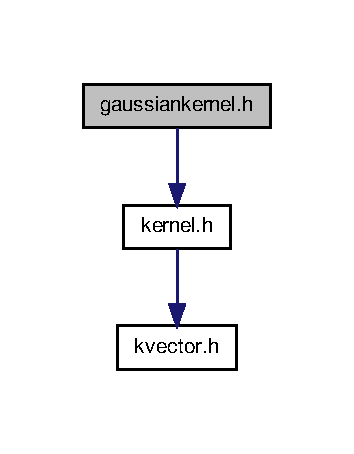
\includegraphics[width=170pt]{gaussiankernel_8h__incl}
\end{center}
\end{figure}
\-This graph shows which files directly or indirectly include this file\-:\nopagebreak
\begin{figure}[H]
\begin{center}
\leavevmode
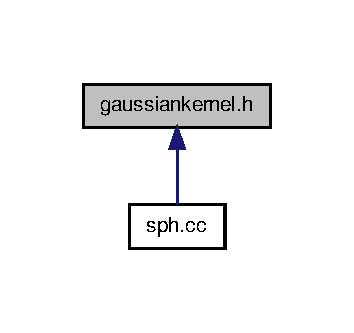
\includegraphics[width=170pt]{gaussiankernel_8h__dep__incl}
\end{center}
\end{figure}
\subsection*{\-Classes}
\begin{DoxyCompactItemize}
\item 
class \hyperlink{classGaussianKernel}{\-Gaussian\-Kernel}
\begin{DoxyCompactList}\small\item\em \-Gaussian approximation of point particle. \end{DoxyCompactList}\end{DoxyCompactItemize}


\subsection{\-Detailed \-Description}
implementation of a \-Gaussian \hyperlink{classKernel}{\-Kernel} 
\hypertarget{incompinvisc_8h}{\section{incompinvisc.\-h \-File \-Reference}
\label{incompinvisc_8h}\index{incompinvisc.\-h@{incompinvisc.\-h}}
}


implementation of \hyperlink{classPhysics}{\-Physics} for a fluid which is incompressible and inviscid  


{\ttfamily \#include \char`\"{}physics.\-h\char`\"{}}\*
{\ttfamily \#include \char`\"{}properties.\-h\char`\"{}}\*
{\ttfamily \#include \char`\"{}kvector.\-h\char`\"{}}\*
\-Include dependency graph for incompinvisc.\-h\-:\nopagebreak
\begin{figure}[H]
\begin{center}
\leavevmode
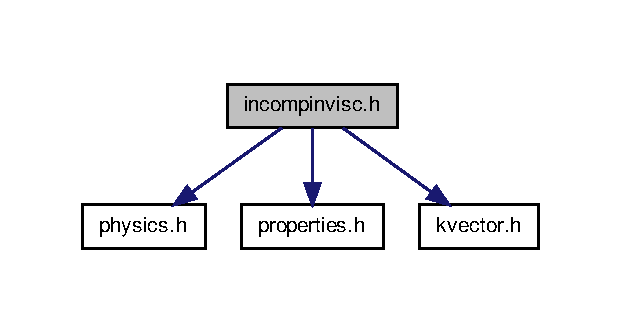
\includegraphics[width=298pt]{incompinvisc_8h__incl}
\end{center}
\end{figure}
\-This graph shows which files directly or indirectly include this file\-:\nopagebreak
\begin{figure}[H]
\begin{center}
\leavevmode
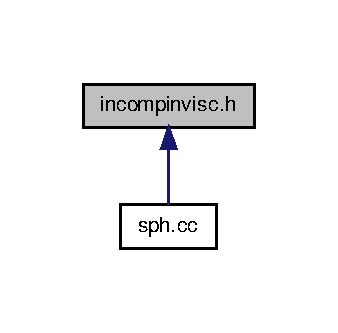
\includegraphics[width=162pt]{incompinvisc_8h__dep__incl}
\end{center}
\end{figure}
\subsection*{\-Classes}
\begin{DoxyCompactItemize}
\item 
class \hyperlink{classIncompInvisc}{\-Incomp\-Invisc}
\begin{DoxyCompactList}\small\item\em class for an incompressibe, inviscid fluid \end{DoxyCompactList}\end{DoxyCompactItemize}


\subsection{\-Detailed \-Description}
implementation of \hyperlink{classPhysics}{\-Physics} for a fluid which is incompressible and inviscid 
\hypertarget{incompvisc_8h}{\section{incompvisc.\-h \-File \-Reference}
\label{incompvisc_8h}\index{incompvisc.\-h@{incompvisc.\-h}}
}


implementation of physics for a fluid which is incompressible and inviscid  


{\ttfamily \#include \char`\"{}physics.\-h\char`\"{}}\*
{\ttfamily \#include \char`\"{}properties.\-h\char`\"{}}\*
{\ttfamily \#include \char`\"{}kvector.\-h\char`\"{}}\*
{\ttfamily \#include \char`\"{}fluid.\-h\char`\"{}}\*
{\ttfamily \#include \char`\"{}particle.\-h\char`\"{}}\*
{\ttfamily \#include \char`\"{}kernel.\-h\char`\"{}}\*
{\ttfamily \#include $<$cmath$>$}\*
\subsection*{\-Classes}
\begin{DoxyCompactItemize}
\item 
class \hyperlink{classIncompVisc}{\-Incomp\-Visc}
\begin{DoxyCompactList}\small\item\em class for an incompressible fluid with the inclusion of viscous forces \end{DoxyCompactList}\end{DoxyCompactItemize}


\subsection{\-Detailed \-Description}
implementation of physics for a fluid which is incompressible and inviscid 
\hypertarget{initialize_8h}{\section{initialize.\-h \-File \-Reference}
\label{initialize_8h}\index{initialize.\-h@{initialize.\-h}}
}


\-Code for initialization of fluid and boundary from input files.  


{\ttfamily \#include $<$string$>$}\*
{\ttfamily \#include $<$stdio.\-h$>$}\*
\-Include dependency graph for initialize.\-h\-:\nopagebreak
\begin{figure}[H]
\begin{center}
\leavevmode
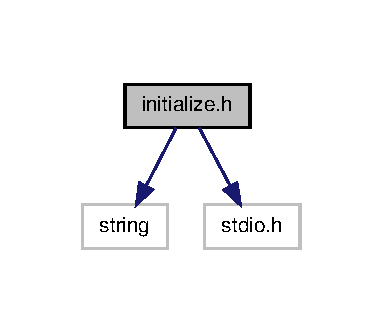
\includegraphics[width=184pt]{initialize_8h__incl}
\end{center}
\end{figure}
\-This graph shows which files directly or indirectly include this file\-:\nopagebreak
\begin{figure}[H]
\begin{center}
\leavevmode
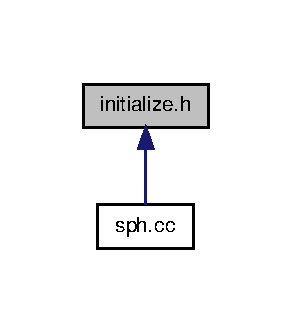
\includegraphics[width=140pt]{initialize_8h__dep__incl}
\end{center}
\end{figure}
\subsection*{\-Functions}
\begin{DoxyCompactItemize}
\item 
bool \hyperlink{initialize_8h_adc785f0a8be92a49a45c287c8e001901}{get\-Nparticles} (const std\-::string \&filename, const std\-::string \&boundary\-File, int \&nparticles, int \&nboundaries)
\begin{DoxyCompactList}\small\item\em find the number of particles and boundary particles from input files \end{DoxyCompactList}\item 
bool \hyperlink{initialize_8h_aed9e1abd9c526bb27fcbd370c820fe30}{initialize} (const std\-::string \&filename, const std\-::string \&boundary\-File, \hyperlink{classFluid}{\-Fluid} \&fluid, int \&nparticles, int \&nboundaries)
\begin{DoxyCompactList}\small\item\em initializes fluid from input files \end{DoxyCompactList}\item 
void \hyperlink{initialize_8h_af1eddf5f8dbfa62cdf6637f86467531e}{rectangle\-Particles} (\hyperlink{structKvector}{\-Kvector} p0, \hyperlink{structKvector}{\-Kvector} p1, double density, double smoothinglength, \hyperlink{classFluid}{\-Fluid} \&fluid)
\begin{DoxyCompactList}\small\item\em alternate initialization of fluid in a rectangle \end{DoxyCompactList}\end{DoxyCompactItemize}


\subsection{\-Detailed \-Description}
\-Code for initialization of fluid and boundary from input files. 

\subsection{\-Function \-Documentation}
\hypertarget{initialize_8h_adc785f0a8be92a49a45c287c8e001901}{\index{initialize.\-h@{initialize.\-h}!get\-Nparticles@{get\-Nparticles}}
\index{get\-Nparticles@{get\-Nparticles}!initialize.h@{initialize.\-h}}
\subsubsection[{get\-Nparticles}]{\setlength{\rightskip}{0pt plus 5cm}bool {\bf get\-Nparticles} (
\begin{DoxyParamCaption}
\item[{const std\-::string \&}]{filename, }
\item[{const std\-::string \&}]{boundary\-File, }
\item[{int \&}]{nparticles, }
\item[{int \&}]{nboundaries}
\end{DoxyParamCaption}
)}}\label{initialize_8h_adc785f0a8be92a49a45c287c8e001901}


find the number of particles and boundary particles from input files 


\begin{DoxyParams}{\-Parameters}
{\em filename} & file with initial particle properties \\
\hline
{\em boundary\-File} & file with initial boundary particle properties \\
\hline
{\em nparticles} & address for number of particles \\
\hline
{\em nboundaries} & address for number of boundary particles \\
\hline
\end{DoxyParams}
\hypertarget{initialize_8h_aed9e1abd9c526bb27fcbd370c820fe30}{\index{initialize.\-h@{initialize.\-h}!initialize@{initialize}}
\index{initialize@{initialize}!initialize.h@{initialize.\-h}}
\subsubsection[{initialize}]{\setlength{\rightskip}{0pt plus 5cm}bool {\bf initialize} (
\begin{DoxyParamCaption}
\item[{const std\-::string \&}]{filename, }
\item[{const std\-::string \&}]{boundary\-File, }
\item[{{\bf \-Fluid} \&}]{fluid, }
\item[{int \&}]{nparticles, }
\item[{int \&}]{nboundaries}
\end{DoxyParamCaption}
)}}\label{initialize_8h_aed9e1abd9c526bb27fcbd370c820fe30}


initializes fluid from input files 


\begin{DoxyParams}{\-Parameters}
{\em filename} & file with initial particle properties \\
\hline
{\em boundary\-File} & file with initial boundary particle properties \\
\hline
{\em fluid} & fluid to be initialized \\
\hline
{\em nparticles} & address for number of particles \\
\hline
{\em nboundaries} & address for number of boundary particles \\
\hline
\end{DoxyParams}
\hypertarget{initialize_8h_af1eddf5f8dbfa62cdf6637f86467531e}{\index{initialize.\-h@{initialize.\-h}!rectangle\-Particles@{rectangle\-Particles}}
\index{rectangle\-Particles@{rectangle\-Particles}!initialize.h@{initialize.\-h}}
\subsubsection[{rectangle\-Particles}]{\setlength{\rightskip}{0pt plus 5cm}void {\bf rectangle\-Particles} (
\begin{DoxyParamCaption}
\item[{{\bf \-Kvector}}]{p0, }
\item[{{\bf \-Kvector}}]{p1, }
\item[{double}]{density, }
\item[{double}]{smoothinglength, }
\item[{{\bf \-Fluid} \&}]{fluid}
\end{DoxyParamCaption}
)}}\label{initialize_8h_af1eddf5f8dbfa62cdf6637f86467531e}


alternate initialization of fluid in a rectangle 


\begin{DoxyParams}{\-Parameters}
{\em p0} & bottom left corner of fluid rectangle \\
\hline
{\em p1} & top right corner of fluid rectangle \\
\hline
{\em density} & initial density of particles \\
\hline
{\em smoothinglength} & smoothing length \\
\hline
{\em fluid} & fluid to be initialized \\
\hline
\end{DoxyParams}

\hypertarget{integrator_8h}{\section{integrator.\-h \-File \-Reference}
\label{integrator_8h}\index{integrator.\-h@{integrator.\-h}}
}


superclass for integrators  


\-This graph shows which files directly or indirectly include this file\-:
\nopagebreak
\begin{figure}[H]
\begin{center}
\leavevmode
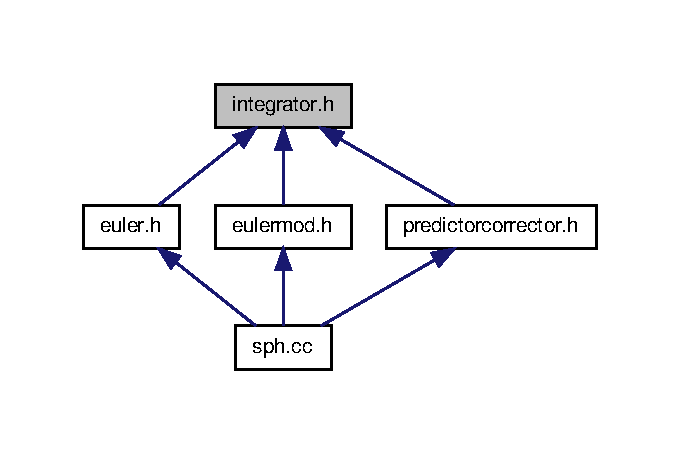
\includegraphics[width=244pt]{integrator_8h__dep__incl}
\end{center}
\end{figure}
\subsection*{\-Classes}
\begin{DoxyCompactItemize}
\item 
class \hyperlink{classIntegrator}{\-Integrator}
\begin{DoxyCompactList}\small\item\em superclass for integrators \end{DoxyCompactList}\end{DoxyCompactItemize}


\subsection{\-Detailed \-Description}
superclass for integrators 
\hypertarget{kernel_8h}{\section{kernel.\-h \-File \-Reference}
\label{kernel_8h}\index{kernel.\-h@{kernel.\-h}}
}


superclass for kernels  


{\ttfamily \#include \char`\"{}kvector.\-h\char`\"{}}\*
\-Include dependency graph for kernel.\-h\-:
\nopagebreak
\begin{figure}[H]
\begin{center}
\leavevmode
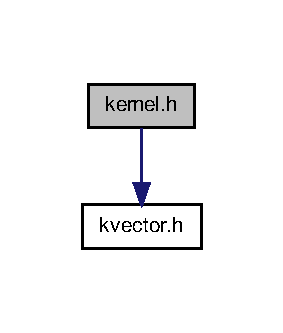
\includegraphics[width=136pt]{kernel_8h__incl}
\end{center}
\end{figure}
\-This graph shows which files directly or indirectly include this file\-:
\nopagebreak
\begin{figure}[H]
\begin{center}
\leavevmode
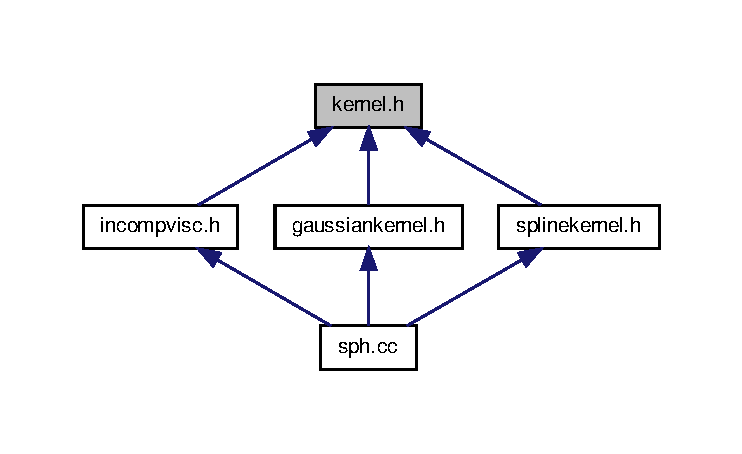
\includegraphics[width=350pt]{kernel_8h__dep__incl}
\end{center}
\end{figure}
\subsection*{\-Classes}
\begin{DoxyCompactItemize}
\item 
class \hyperlink{classKernel}{\-Kernel}
\begin{DoxyCompactList}\small\item\em smooth kernels approximating point particles \end{DoxyCompactList}\end{DoxyCompactItemize}


\subsection{\-Detailed \-Description}
superclass for kernels 
\hypertarget{kernel__test_8cc}{\section{kernel\-\_\-test.\-cc \-File \-Reference}
\label{kernel__test_8cc}\index{kernel\-\_\-test.\-cc@{kernel\-\_\-test.\-cc}}
}


\-Tests \hyperlink{classSplineKernel}{\-Spline\-Kernel} and \hyperlink{classGaussianKernel}{\-Gaussian\-Kernel}.  


{\ttfamily \#include \char`\"{}kernel\-\_\-test.\-h\char`\"{}}\*
\-Include dependency graph for kernel\-\_\-test.\-cc\-:\nopagebreak
\begin{figure}[H]
\begin{center}
\leavevmode
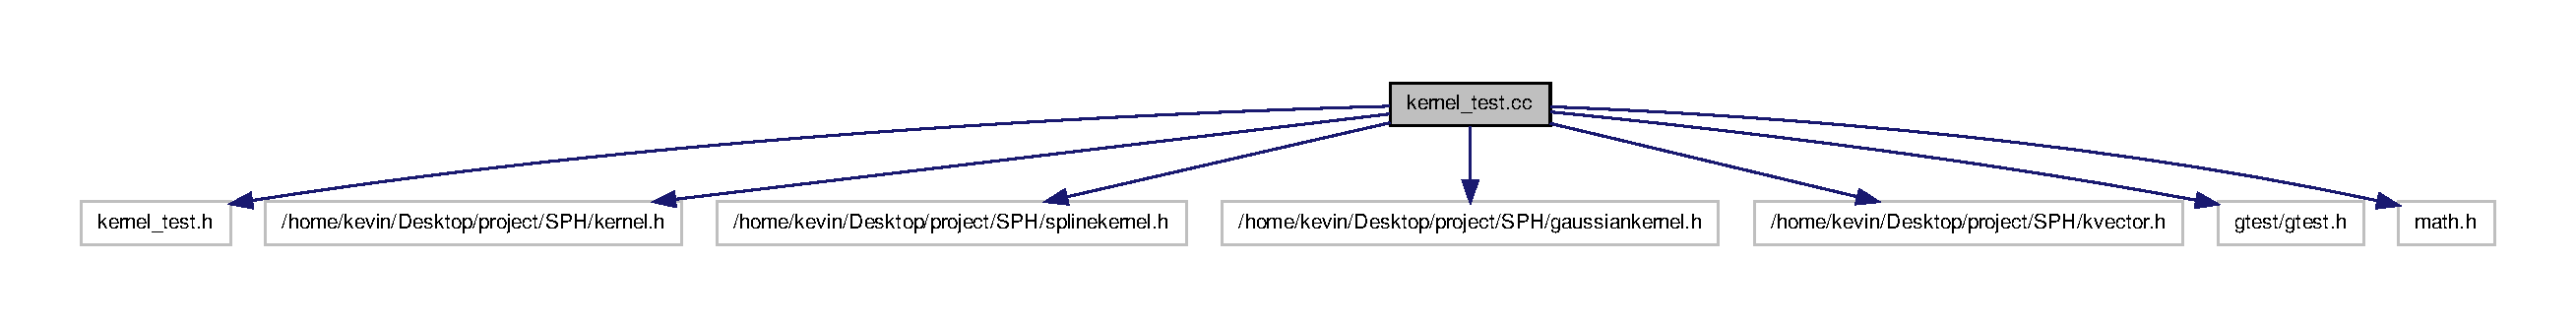
\includegraphics[width=350pt]{kernel__test_8cc__incl}
\end{center}
\end{figure}
\subsection*{\-Functions}
\begin{DoxyCompactItemize}
\item 
\hypertarget{kernel__test_8cc_afd251b12d546a8f7d9209a42adb331c0}{\hyperlink{kernel__test_8cc_afd251b12d546a8f7d9209a42adb331c0}{\-T\-E\-S\-T\-\_\-\-F} (\-Kernel\-Test, gaussian\-W)}\label{kernel__test_8cc_afd251b12d546a8f7d9209a42adb331c0}

\begin{DoxyCompactList}\small\item\em tests \hyperlink{classGaussianKernel_ae6d613700d1d59f463094cc5c43ce97c}{\-Gaussian\-Kernel\-::\-W} \end{DoxyCompactList}\item 
\hypertarget{kernel__test_8cc_a83bf0e91e98cdc621878e5d3951e6235}{\hyperlink{kernel__test_8cc_a83bf0e91e98cdc621878e5d3951e6235}{\-T\-E\-S\-T\-\_\-\-F} (\-Kernel\-Test, spline\-W)}\label{kernel__test_8cc_a83bf0e91e98cdc621878e5d3951e6235}

\begin{DoxyCompactList}\small\item\em tests \hyperlink{classSplineKernel_a8dd3d968b0436c799789da0777398151}{\-Spline\-Kernel\-::\-W} \end{DoxyCompactList}\item 
\hypertarget{kernel__test_8cc_a2e5554c297b90c0554e81dcc5dec9019}{\hyperlink{kernel__test_8cc_a2e5554c297b90c0554e81dcc5dec9019}{\-T\-E\-S\-T\-\_\-\-F} (\-Kernel\-Test, gaussian\-Grad\-W)}\label{kernel__test_8cc_a2e5554c297b90c0554e81dcc5dec9019}

\begin{DoxyCompactList}\small\item\em tests \-Gaussian\-Kernel\-::\-Grad\-W \end{DoxyCompactList}\item 
\hypertarget{kernel__test_8cc_a5c2f2f55e78e9ed479149112c19cf380}{\hyperlink{kernel__test_8cc_a5c2f2f55e78e9ed479149112c19cf380}{\-T\-E\-S\-T\-\_\-\-F} (\-Kernel\-Test, spline\-Grad\-W)}\label{kernel__test_8cc_a5c2f2f55e78e9ed479149112c19cf380}

\begin{DoxyCompactList}\small\item\em tests \-Spline\-Kernel\-::\-Grad\-W \end{DoxyCompactList}\end{DoxyCompactItemize}


\subsection{\-Detailed \-Description}
\-Tests \hyperlink{classSplineKernel}{\-Spline\-Kernel} and \hyperlink{classGaussianKernel}{\-Gaussian\-Kernel}. 
\hypertarget{kvector_8h}{\section{kvector.\-h \-File \-Reference}
\label{kvector_8h}\index{kvector.\-h@{kvector.\-h}}
}


struct for 2\-D vector object useful for kernel operations  


\-This graph shows which files directly or indirectly include this file\-:
\nopagebreak
\begin{figure}[H]
\begin{center}
\leavevmode
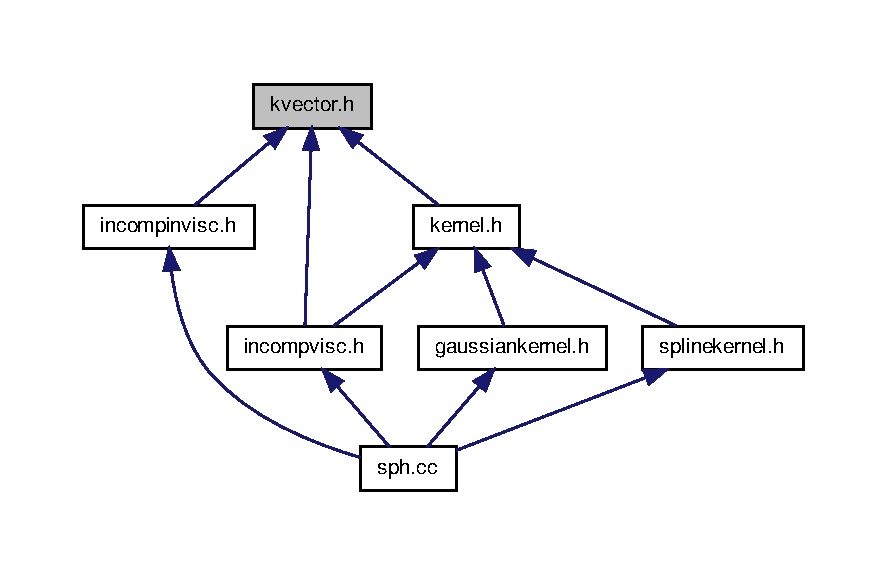
\includegraphics[width=350pt]{kvector_8h__dep__incl}
\end{center}
\end{figure}
\subsection*{\-Classes}
\begin{DoxyCompactItemize}
\item 
struct \hyperlink{structKvector}{\-Kvector}
\begin{DoxyCompactList}\small\item\em struct for 2\-D vector useful for kernel operations \end{DoxyCompactList}\end{DoxyCompactItemize}


\subsection{\-Detailed \-Description}
struct for 2\-D vector object useful for kernel operations 
\hypertarget{kvector__test_8cc}{\section{kvector\-\_\-test.\-cc \-File \-Reference}
\label{kvector__test_8cc}\index{kvector\-\_\-test.\-cc@{kvector\-\_\-test.\-cc}}
}


tests for \hyperlink{structKvector}{\-Kvector}  


{\ttfamily \#include \char`\"{}kvector\-\_\-test.\-h\char`\"{}}\*
\subsection*{\-Functions}
\begin{DoxyCompactItemize}
\item 
\hypertarget{kvector__test_8cc_a84e1abf6483b3b2da36f5d05b2ad7cc1}{{\bfseries \-T\-E\-S\-T} (\-Kvector\-Test, kvector)}\label{kvector__test_8cc_a84e1abf6483b3b2da36f5d05b2ad7cc1}

\end{DoxyCompactItemize}


\subsection{\-Detailed \-Description}
tests for \hyperlink{structKvector}{\-Kvector} 
\hypertarget{output_8h}{\section{output.\-h \-File \-Reference}
\label{output_8h}\index{output.\-h@{output.\-h}}
}


\-Class which outputs current fluid state.  


{\ttfamily \#include $<$fstream$>$}\*
\subsection*{\-Classes}
\begin{DoxyCompactItemize}
\item 
class \hyperlink{classOutput}{\-Output}
\begin{DoxyCompactList}\small\item\em \-Class to build output file for fluid state. \end{DoxyCompactList}\end{DoxyCompactItemize}


\subsection{\-Detailed \-Description}
\-Class which outputs current fluid state. 
\hypertarget{particle_8h}{\section{particle.\-h \-File \-Reference}
\label{particle_8h}\index{particle.\-h@{particle.\-h}}
}


\-Definition of the particle class.  


{\ttfamily \#include $<$string$>$}\*
{\ttfamily \#include $<$vector$>$}\*
{\ttfamily \#include \char`\"{}properties.\-h\char`\"{}}\*
\-Include dependency graph for particle.\-h\-:\nopagebreak
\begin{figure}[H]
\begin{center}
\leavevmode
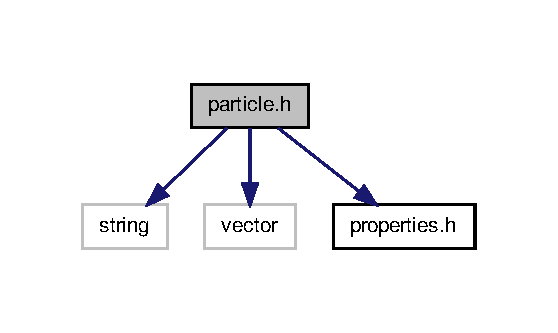
\includegraphics[width=268pt]{particle_8h__incl}
\end{center}
\end{figure}
\-This graph shows which files directly or indirectly include this file\-:\nopagebreak
\begin{figure}[H]
\begin{center}
\leavevmode
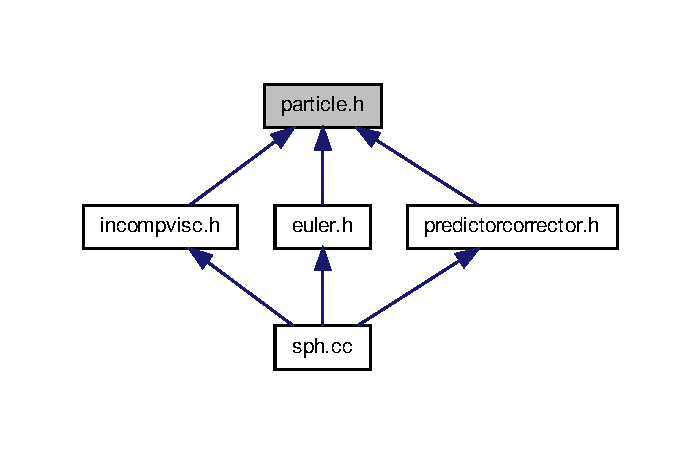
\includegraphics[width=350pt]{particle_8h__dep__incl}
\end{center}
\end{figure}
\subsection*{\-Classes}
\begin{DoxyCompactItemize}
\item 
class \hyperlink{classParticle}{\-Particle}
\begin{DoxyCompactList}\small\item\em \hyperlink{structProperties}{\-Properties} and functions for individual particles. \end{DoxyCompactList}\end{DoxyCompactItemize}


\subsection{\-Detailed \-Description}
\-Definition of the particle class. 
\hypertarget{particle__test_8cc}{\section{particle\-\_\-test.\-cc \-File \-Reference}
\label{particle__test_8cc}\index{particle\-\_\-test.\-cc@{particle\-\_\-test.\-cc}}
}


tests \hyperlink{classParticle}{\-Particle}  


{\ttfamily \#include \char`\"{}particle\-\_\-test.\-h\char`\"{}}\*
\subsection*{\-Functions}
\begin{DoxyCompactItemize}
\item 
\hypertarget{particle__test_8cc_a7a293117d36c8787a7ffb1cee6160431}{\hyperlink{particle__test_8cc_a7a293117d36c8787a7ffb1cee6160431}{\-T\-E\-S\-T\-\_\-\-F} (\-Particle\-Test, check\-Get\-Set)}\label{particle__test_8cc_a7a293117d36c8787a7ffb1cee6160431}

\begin{DoxyCompactList}\small\item\em tests \hyperlink{classParticle_ac2bd006400deb1c9f17ddce9d70d3728}{\-Particle\-::get\-Old\-Properties} and \hyperlink{classParticle_afea2eefc83b471a45c9b1e6c442b91c6}{\-Particle\-::set\-New\-Properties} \end{DoxyCompactList}\item 
\hypertarget{particle__test_8cc_a9fb495ed0a5d3da06f0e25d16d8847c0}{\hyperlink{particle__test_8cc_a9fb495ed0a5d3da06f0e25d16d8847c0}{\-T\-E\-S\-T\-\_\-\-F} (\-Particle\-Test, check\-Neighbors)}\label{particle__test_8cc_a9fb495ed0a5d3da06f0e25d16d8847c0}

\begin{DoxyCompactList}\small\item\em tests \hyperlink{classParticle_addaece13cd072de3db9b3281262a9793}{\-Particle\-::number\-Of\-Neighbors}, \hyperlink{classParticle_a3ac6511d98e8472de59bb474dfe851a1}{\-Particle\-::add\-Neighbor}, \hyperlink{classParticle_a54b1e463538ca132ca86c758ca1f04c2}{\-Particle\-::delete\-Neighbors} \end{DoxyCompactList}\item 
\hypertarget{particle__test_8cc_a23f80e165b278c7d38f36fa0e0b60b3d}{\hyperlink{particle__test_8cc_a23f80e165b278c7d38f36fa0e0b60b3d}{\-T\-E\-S\-T\-\_\-\-F} (\-Particle\-Test, check\-Get\-Tag)}\label{particle__test_8cc_a23f80e165b278c7d38f36fa0e0b60b3d}

\begin{DoxyCompactList}\small\item\em tests \hyperlink{classParticle_adce0a40cce7f7862ff2fc0e6bab2e3f4}{\-Particle\-::get\-Tag} \end{DoxyCompactList}\end{DoxyCompactItemize}


\subsection{\-Detailed \-Description}
tests \hyperlink{classParticle}{\-Particle} 
\hypertarget{physics_8h}{\section{physics.\-h \-File \-Reference}
\label{physics_8h}\index{physics.\-h@{physics.\-h}}
}


superclass for implementing different fluid physics  


\-This graph shows which files directly or indirectly include this file\-:\nopagebreak
\begin{figure}[H]
\begin{center}
\leavevmode
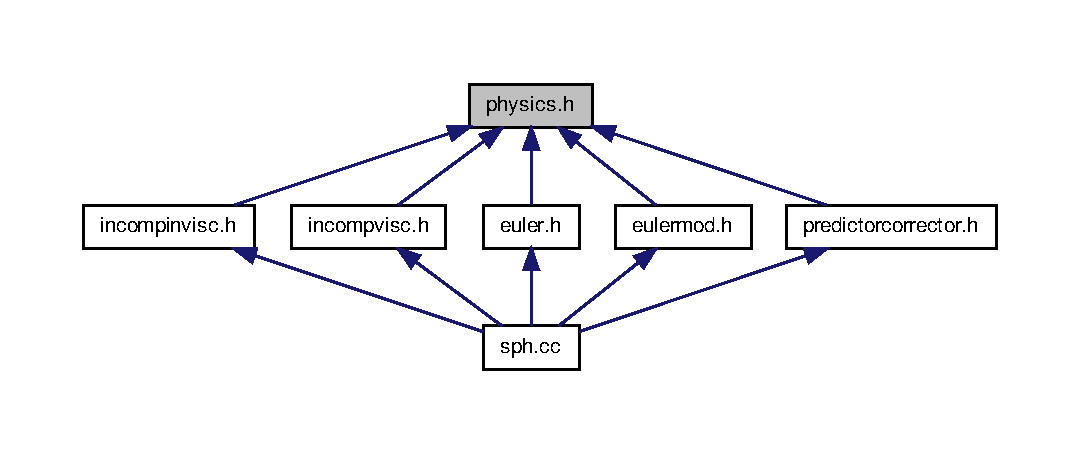
\includegraphics[width=350pt]{physics_8h__dep__incl}
\end{center}
\end{figure}
\subsection*{\-Classes}
\begin{DoxyCompactItemize}
\item 
class \hyperlink{classPhysics}{\-Physics}
\begin{DoxyCompactList}\small\item\em superclass for implementing different fluid physics \end{DoxyCompactList}\end{DoxyCompactItemize}


\subsection{\-Detailed \-Description}
superclass for implementing different fluid physics 
\hypertarget{predictorcorrector_8h}{\section{predictorcorrector.\-h \-File \-Reference}
\label{predictorcorrector_8h}\index{predictorcorrector.\-h@{predictorcorrector.\-h}}
}


\hyperlink{classIntegrator}{\-Integrator} implementing the modified predictor-\/corrector method outlined in \-Price (2004).  


{\ttfamily \#include \char`\"{}integrator.\-h\char`\"{}}\*
{\ttfamily \#include \char`\"{}fluid.\-h\char`\"{}}\*
{\ttfamily \#include \char`\"{}physics.\-h\char`\"{}}\*
{\ttfamily \#include \char`\"{}particle.\-h\char`\"{}}\*
\-Include dependency graph for predictorcorrector.\-h\-:\nopagebreak
\begin{figure}[H]
\begin{center}
\leavevmode
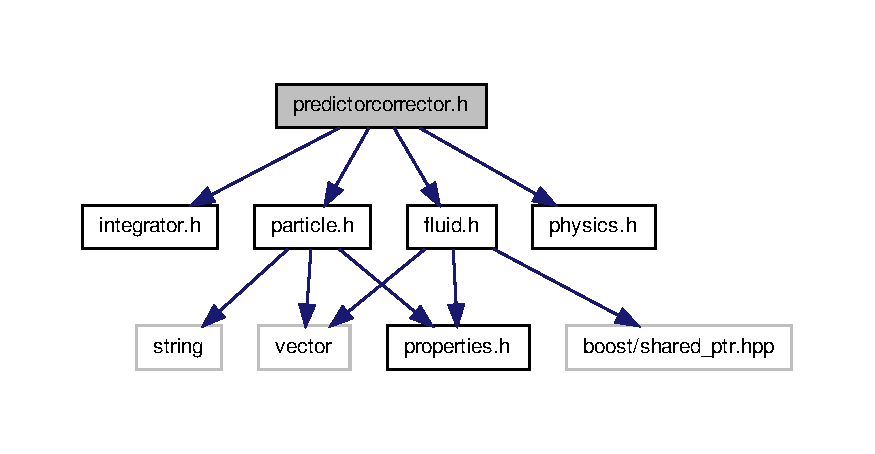
\includegraphics[width=350pt]{predictorcorrector_8h__incl}
\end{center}
\end{figure}
\-This graph shows which files directly or indirectly include this file\-:\nopagebreak
\begin{figure}[H]
\begin{center}
\leavevmode
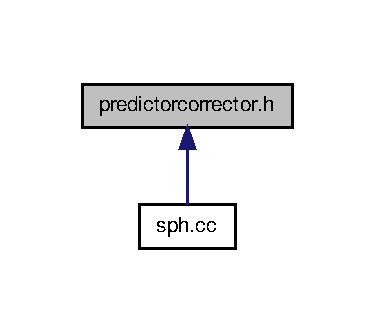
\includegraphics[width=180pt]{predictorcorrector_8h__dep__incl}
\end{center}
\end{figure}
\subsection*{\-Classes}
\begin{DoxyCompactItemize}
\item 
class \hyperlink{classPredictorCorrector}{\-Predictor\-Corrector}
\begin{DoxyCompactList}\small\item\em \-Predictor-\/corrector integrator. \end{DoxyCompactList}\end{DoxyCompactItemize}


\subsection{\-Detailed \-Description}
\hyperlink{classIntegrator}{\-Integrator} implementing the modified predictor-\/corrector method outlined in \-Price (2004). 
\hypertarget{properties_8h}{\section{properties.\-h \-File \-Reference}
\label{properties_8h}\index{properties.\-h@{properties.\-h}}
}


\-Struct to hold a particle's physical properties.  


\-This graph shows which files directly or indirectly include this file\-:
\nopagebreak
\begin{figure}[H]
\begin{center}
\leavevmode
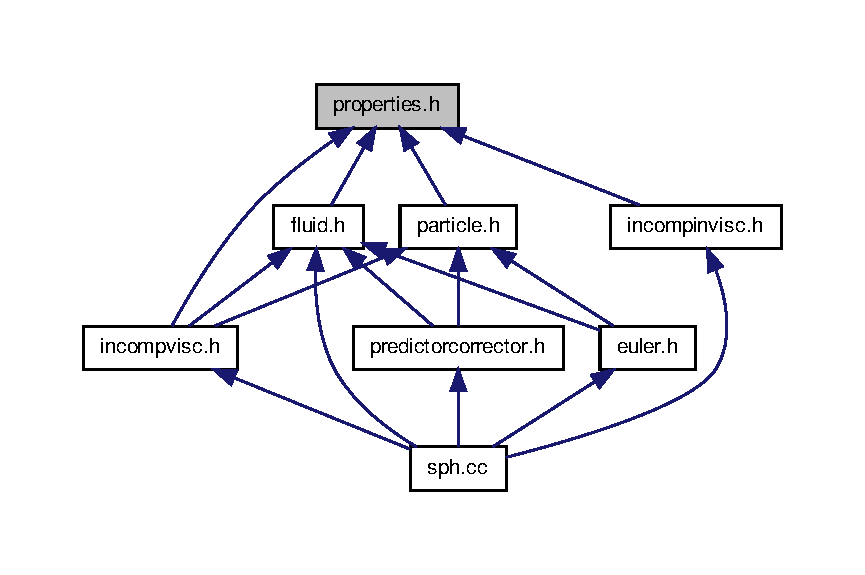
\includegraphics[width=350pt]{properties_8h__dep__incl}
\end{center}
\end{figure}
\subsection*{\-Classes}
\begin{DoxyCompactItemize}
\item 
struct \hyperlink{structProperties}{\-Properties}
\begin{DoxyCompactList}\small\item\em struct holding physical particle properties \end{DoxyCompactList}\end{DoxyCompactItemize}


\subsection{\-Detailed \-Description}
\-Struct to hold a particle's physical properties. 
\hypertarget{properties__test_8cc}{\section{properties\-\_\-test.\-cc \-File \-Reference}
\label{properties__test_8cc}\index{properties\-\_\-test.\-cc@{properties\-\_\-test.\-cc}}
}


\-Tests for \hyperlink{structProperties}{\-Properties}.  


{\ttfamily \#include \char`\"{}properties\-\_\-test.\-h\char`\"{}}\*
\subsection*{\-Functions}
\begin{DoxyCompactItemize}
\item 
\hypertarget{properties__test_8cc_a76b55472205315e03c46be4a414a5316}{\hyperlink{properties__test_8cc_a76b55472205315e03c46be4a414a5316}{\-T\-E\-S\-T} (\-Properties\-Test, check\-All\-Props)}\label{properties__test_8cc_a76b55472205315e03c46be4a414a5316}

\begin{DoxyCompactList}\small\item\em tests that \hyperlink{structProperties}{\-Properties} initializes properly \end{DoxyCompactList}\end{DoxyCompactItemize}


\subsection{\-Detailed \-Description}
\-Tests for \hyperlink{structProperties}{\-Properties}. 
\hypertarget{sph_8cc}{\section{sph.\-cc \-File \-Reference}
\label{sph_8cc}\index{sph.\-cc@{sph.\-cc}}
}


\-Driver program for smoothed particle hydrodynamics solver.  


{\ttfamily \#include $<$cstdlib$>$}\*
{\ttfamily \#include $<$iostream$>$}\*
{\ttfamily \#include $<$string$>$}\*
{\ttfamily \#include $<$cmath$>$}\*
{\ttfamily \#include $<$boost/shared\-\_\-ptr.\-hpp$>$}\*
{\ttfamily \#include \char`\"{}fluid.\-h\char`\"{}}\*
{\ttfamily \#include \char`\"{}initialize.\-h\char`\"{}}\*
{\ttfamily \#include \char`\"{}incompinvisc.\-h\char`\"{}}\*
{\ttfamily \#include \char`\"{}incompvisc.\-h\char`\"{}}\*
{\ttfamily \#include \char`\"{}gaussiankernel.\-h\char`\"{}}\*
{\ttfamily \#include \char`\"{}splinekernel.\-h\char`\"{}}\*
{\ttfamily \#include \char`\"{}euler.\-h\char`\"{}}\*
{\ttfamily \#include \char`\"{}eulermod.\-h\char`\"{}}\*
{\ttfamily \#include \char`\"{}predictorcorrector.\-h\char`\"{}}\*
{\ttfamily \#include \char`\"{}output.\-h\char`\"{}}\*
\-Include dependency graph for sph.\-cc\-:
\nopagebreak
\begin{figure}[H]
\begin{center}
\leavevmode
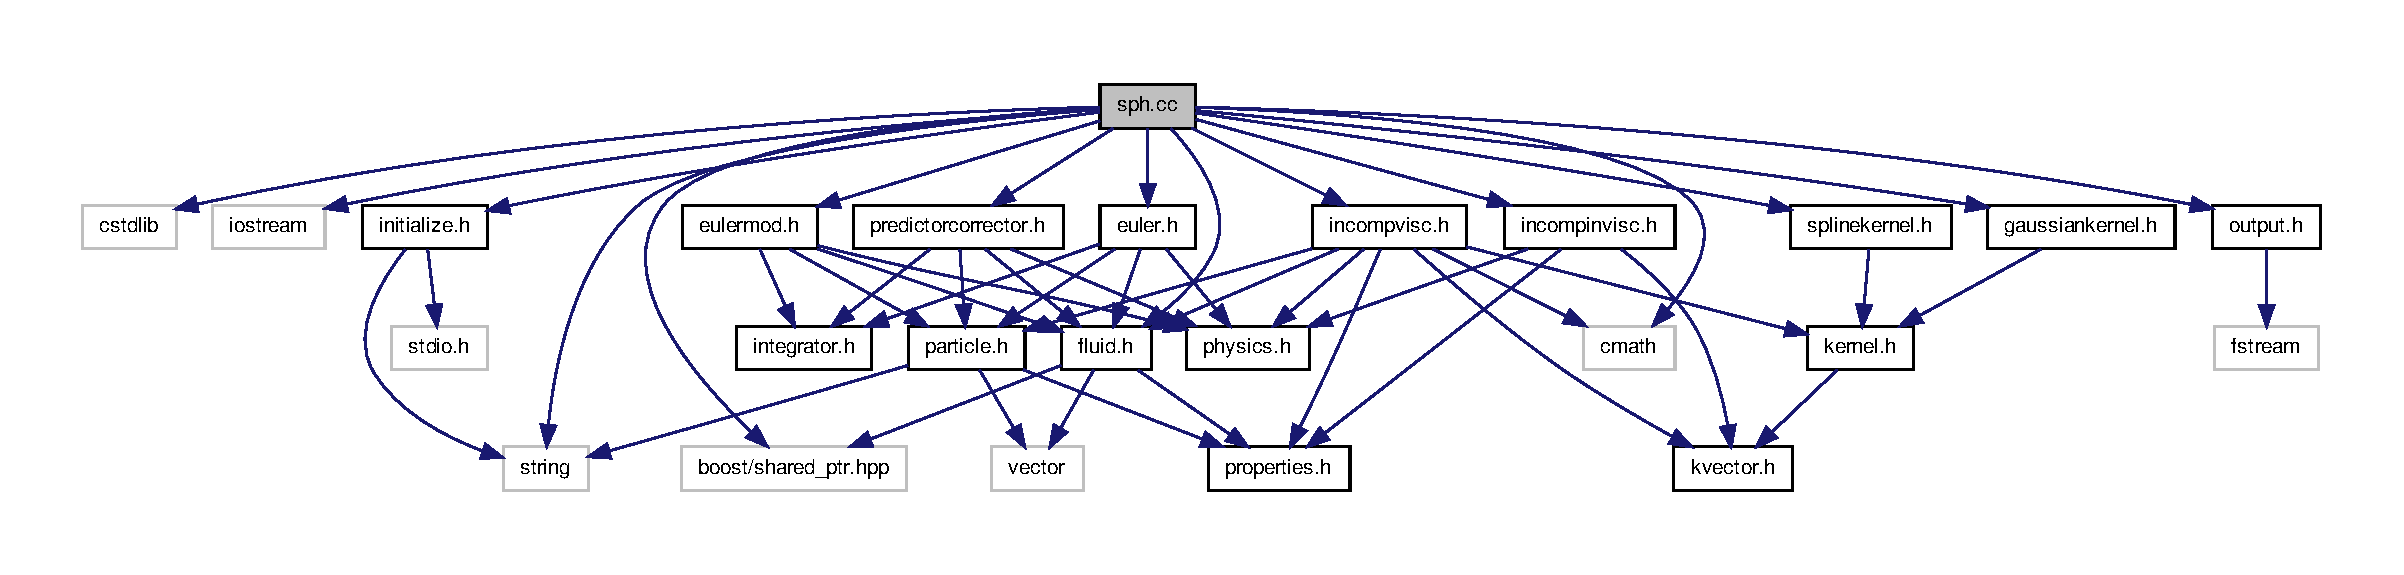
\includegraphics[width=350pt]{sph_8cc__incl}
\end{center}
\end{figure}
\subsection*{\-Functions}
\begin{DoxyCompactItemize}
\item 
\hypertarget{sph_8cc_a3c04138a5bfe5d72780bb7e82a18e627}{int \hyperlink{sph_8cc_a3c04138a5bfe5d72780bb7e82a18e627}{main} (int argc, char $\ast$$\ast$argv)}\label{sph_8cc_a3c04138a5bfe5d72780bb7e82a18e627}

\begin{DoxyCompactList}\small\item\em \-Usage\-: main $<$initial\-File$>$ $<$boundary\-File(\-O\-P\-T\-I\-O\-N\-A\-L)$>$ $<$t\-Final$>$ $<$timestep$>$ \end{DoxyCompactList}\end{DoxyCompactItemize}


\subsection{\-Detailed \-Description}
\-Driver program for smoothed particle hydrodynamics solver. 
\hypertarget{splinekernel_8h}{\section{splinekernel.\-h \-File \-Reference}
\label{splinekernel_8h}\index{splinekernel.\-h@{splinekernel.\-h}}
}


implentation of a cubic spline \hyperlink{classKernel}{\-Kernel}  


{\ttfamily \#include \char`\"{}kernel.\-h\char`\"{}}\*
\-Include dependency graph for splinekernel.\-h\-:\nopagebreak
\begin{figure}[H]
\begin{center}
\leavevmode
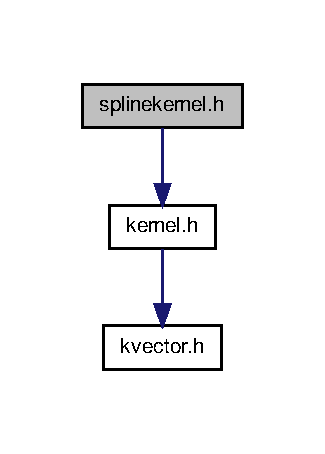
\includegraphics[width=156pt]{splinekernel_8h__incl}
\end{center}
\end{figure}
\-This graph shows which files directly or indirectly include this file\-:\nopagebreak
\begin{figure}[H]
\begin{center}
\leavevmode
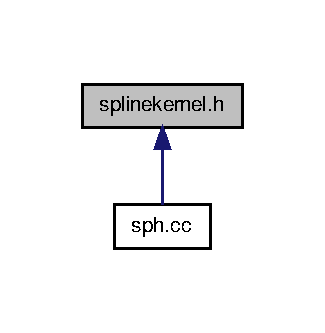
\includegraphics[width=156pt]{splinekernel_8h__dep__incl}
\end{center}
\end{figure}
\subsection*{\-Classes}
\begin{DoxyCompactItemize}
\item 
class \hyperlink{classSplineKernel}{\-Spline\-Kernel}
\begin{DoxyCompactList}\small\item\em cubic spline approximation of point particle \end{DoxyCompactList}\end{DoxyCompactItemize}


\subsection{\-Detailed \-Description}
implentation of a cubic spline \hyperlink{classKernel}{\-Kernel} 
\hypertarget{tests_8cc}{\section{tests.\-cc \-File \-Reference}
\label{tests_8cc}\index{tests.\-cc@{tests.\-cc}}
}


\-Driver program for testing of sph.  


{\ttfamily \#include $<$stdlib.\-h$>$}\*
{\ttfamily \#include $<$iostream$>$}\*
{\ttfamily \#include \char`\"{}gtest/gtest.\-h\char`\"{}}\*
\-Include dependency graph for tests.\-cc\-:\nopagebreak
\begin{figure}[H]
\begin{center}
\leavevmode
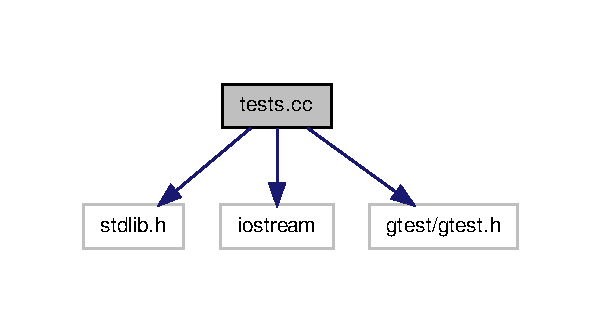
\includegraphics[width=288pt]{tests_8cc__incl}
\end{center}
\end{figure}
\subsection*{\-Functions}
\begin{DoxyCompactItemize}
\item 
\hypertarget{tests_8cc_a3c04138a5bfe5d72780bb7e82a18e627}{int {\bfseries main} (int argc, char $\ast$$\ast$argv)}\label{tests_8cc_a3c04138a5bfe5d72780bb7e82a18e627}

\end{DoxyCompactItemize}


\subsection{\-Detailed \-Description}
\-Driver program for testing of sph. 
\printindex
\end{document}
